\documentclass[letterpaper,12pt,onecolumn,final]{report}

\pdftrailerid{}
\pdfsuppressptexinfo15
\pdfminorversion=4

%% MANDATORY PACKAGES
\usepackage{cuthesis}         % Concordia's thesis style
\usepackage[english]{babel}   % load english localization
\usepackage{type1ec}          % type 1 font
\usepackage[T1]{fontenc}      % correct some font representation, needs cm-super fonts
\usepackage{times}            % use Times New Roman font
\usepackage[titletoc,title]{appendix}     % include Appendix command, add to ToC
\usepackage{setspace}         % control double/single line spacing
\usepackage[pdftex]{graphicx}
\usepackage{caption,tabularx,booktabs}
\usepackage{array}
\usepackage{csquotes}
\newcolumntype{C}[1]{>{\centering\arraybackslash}p{#1}}
%% OPTIONAL PACKAGES
%\counterwithout{footnote}{chapter}        % do no reset footnote # between chapters
\usepackage[hyphens]{url}     % print links
\usepackage{hyperref}         % provides hyperlinks (text different than link)
%\usepackage[hyphenbreaks]{breakurl}       % break long URL after hyphens
\hypersetup{
	colorlinks=true,
	breaklinks=true,
	linkcolor=black,
	citecolor=black,
	urlcolor=black,
	filecolor=black,
	linktoc=all,
}
\usepackage{graphicx}
%\graphicspath{{img/}}


\usepackage{blindtext}

\usepackage{multirow}
\usepackage{listings}
\usepackage{algorithm}
\usepackage{algpseudocode}
\usepackage[section]{placeins}
\usepackage{pgfplots}
\usepackage{pgfplotstable}
\usepackage{filecontents}

%% CUSTOM MACROS
\usepackage{xspace}
\newcommand{\etal}{\textit{et al.}\xspace}
\newcommand{\etc}{\textit{etc.}\xspace}
\newcommand{\ie}{\textit{i.e.,}\xspace}
\newcommand{\eg}{\textit{e.g.,}\xspace}
\newcommand{\cf}{\textit{cf.}\xspace}
\newcommand{\supra}{\textit{Supra}\xspace}
\newcommand{\nee}{\textit{n\'ee}\xspace}
\newcommand{\aka}{\textit{a.k.a.,}\xspace}


\usepackage{tikz}
\usepackage{forest}

% = = = Arrow -> (\lt)
\newcommand{\lt}{$\rightarrow$\xspace}

% = = = Keywords (kw)
\newcommand{\kw}[1]{\textsf{#1}}

% = = = Colored text (textblue)
\newcommand{\textblue}[1]{\textcolor{blue}{#1}}

\newcommand{\crossmark}{\ensuremath{\times}}
\newcommand{\unknown}{--}

% = = = Compact Lists (compactlist, compactlistn)
\newenvironment{compactlist}
  {\begin{itemize} 
  \setlength{\itemsep}{0pt} 
  \setlength{\parskip}{0pt}} 
  {\end{itemize}}
  
\newenvironment{compactlistn}
  {\begin{enumerate} 
  \setlength{\itemsep}{0pt} 
  \setlength{\parskip}{0pt}} 
  {\end{enumerate}}
  
\renewcommand{\labelitemi}{$\bullet$}
  

%------------------------Crypto----------------------%  

% = = = Zp, Gq and Zq
\newcommand{\Zp}{\mathbb{Z}^{*}_{p}}
\newcommand{\Zq}{\mathbb{Z}_{q}}
\newcommand{\Gq}{\mathbb{G}_{q}}

% = = = Encryption, etc.
\newcommand{\Enc}[1]{\mathsf{Enc}(#1)}
\newcommand{\EncB}[1]{\llbracket #1 \rrbracket}
\newcommand{\ReRand}[1]{\mathsf{ReRand}(#1)}
\newcommand{\Hash}[1]{\mathcal{H}(#1)}
\newcommand{\Sign}[1]{\mathsf{Sig}(#1)}
\newcommand{\Comm}[1]{\mathsf{Comm}(#1)}
\newcommand{\Open}[1]{\mathsf{Open}(#1)}

% = = = Tuples
\newcommand{\tuple}[1]{\left \langle #1 \right \rangle}


%-------------------Custom for Paper----------------------%

% = = = Name
\newcommand{\Name}{\textsf{System Name}\xspace}
\newcommand{\dai}{\textsf{Dai}\xspace}
\newcommand{\cdp}{\textsf{CDP}\xspace}
\newcommand{\vault}{\textsf{Vault}\xspace}

%\newcommand{\tickyes}{{\small\checkmark}}
%\newcommand{\tickno}{{\small$\times$}}
% TABLES:
\usepackage{adjustbox}
\newcommand{\headrow}[1]{\multicolumn{1}{c}{\adjustbox{angle=30,lap=\width-0.5em}{#1}}}
\newcommand{\full}{$\bullet$}
\newcommand{\prt}{$\circ$}
\newcommand{\none}{$\times$}
%% CUSTOM COMMANDS
\newcommand{\etherbase}{{\scshape EtherBase\xspace}}
\newcommand{\slithersimil}{{\scshape Slither-simil\xspace}}
%\newcommand{\subhead}[1]{\noindent{\textbf{#1.}}}
% !TEX root = ../main.tex

%------------------------LNCS----------------------%

%None

%------------------------Packages----------------------%

% = = = Graphics

%\usepackage[table,xcdraw]{xcolor}

% = = = Subfig (note not subfigure)
\usepackage[caption=false,font=footnotesize]{subfig}

% = = = Math Symbols
\usepackage{amsmath}
%\usepackage{amstext,amssymb,amsthm}
\usepackage{bbm}
\usepackage{stmaryrd}
\usepackage{wasysym}
\usepackage{amssymb}
\usepackage{color}
\usepackage{multirow}
\usepackage{rotating}
\usepackage{makecell}
\usepackage{hhline}
% = = = Other
\usepackage{array}
\usepackage{color}
\usepackage[hyphens]{url}

%------------------------END----------------------%  
  


%% THESIS SETTINGS
\author{Sina Pilehchiha}
\title{Improving Reproducibility in Smart Contract Research}

% As of 2019, title is no longer used...
%\titleOfPhDAuthor{Mr.}         % or Ms., Mrs., Miss, etc. (only for PhD's)

% if PhD, uncomment:
%\PhD
% else if Master's, uncomment:
\mastersDegree{Master of Applied Science}

\program{MASc}
%\program{Computer Science}
\dept{The Department\\of\\Electrical and Computer Engineering}
%\dept{The Department\\of\\Computer Science and Software Engineering}

%% See current GPD at https://www.concordia.ca/admissions/graduate/programs/contacts.html
\GpdOrChairOfDept{Dr.\ M. Zahangir Kabir}
\isGpd % Chair by default
%% See current Dean at  https://www.concordia.ca/ginacody/about/leadership/office-dean/dean-of-engineering-and-computer-science.html
\deanOfENCS{Dr.\ Mourad Debbabi} 
\chairOfCommittee{Dr.\ Yousef R. Shayan}
\examinerFirst{Dr.\ }
\examinerSecond{Dr.\ }
\supervisor{Dr. Amir G. Aghdam}
%% Following two lines are required if you have a co-supervisor
\hasCosupervisor
\coSupervisor{Dr. Jeremy Clark}

%% Comment to use current month, needs to match initial submission
\submitmonth{July}
\submityear{2022}
%% Comment if date of defence is unknown yet, fill for final submission
\defencedate{July 31, 2022}


%%%%%%%%%%%%%%%%%%%%%%%%%%%%%%%%%%%%%%%%%%%%%%%%%%%%%%%%%%%%%%%%%%%%%%%%%%%%%%%

\doublespacing
\begin{document}

\definecolor{codegreen}{rgb}{0,0.6,0}
\definecolor{codegray}{rgb}{0.5,0.5,0.5}
\definecolor{codepurple}{rgb}{0.58,0,0.82}
\definecolor{backcolour}{rgb}{0.95,0.95,0.92}

\lstdefinestyle{mystyle}{
    backgroundcolor=\color{backcolour},   
    commentstyle=\color{codegreen},
    keywordstyle=\color{magenta},
    numberstyle=\tiny\color{codegray},
    stringstyle=\color{codepurple},
    basicstyle=\ttfamily\footnotesize,
    breakatwhitespace=false,         
    breaklines=true,                 
    captionpos=b,                    
    keepspaces=true,                 
    numbers=left,                    
    numbersep=5pt,                  
    showspaces=false,                
    showstringspaces=false,
    showtabs=false,                  
    tabsize=2
}

\lstset{style=mystyle}

\definecolor{verylightgray}{rgb}{.97,.97,.97}

\lstdefinelanguage{Solidity}{
	keywords=[1]{address, anonymous, assembly, assert, balance, break, call, callcode, case, catch, class, constant, continue, constructor, contract, debugger, default, delegatecall, delete, do, else, emit, event, experimental, export, external, false, finally, for, function, gas, if, implements, import, in, indexed, instanceof, interface, internal, is, length, library, log0, log1, log2, log3, log4, memory, modifier, msg, new, payable, pragma, private, protected, public, pure, push, require, return, returns, revert, selfdestruct, send, sender, solidity, storage, struct, suicide, super, switch, then, this, throw, transfer, true, try, typeof, using, value, view, while, with, addmod, ecrecover, keccak256, mulmod, ripemd160, sha256, sha3}, % generic keywords including crypto operations
	keywordstyle=[1]\color{blue}\bfseries,
	keywords=[2]{bool, byte, bytes, bytes1, bytes2, bytes3, bytes4, bytes5, bytes6, bytes7, bytes8, bytes9, bytes10, bytes11, bytes12, bytes13, bytes14, bytes15, bytes16, bytes17, bytes18, bytes19, bytes20, bytes21, bytes22, bytes23, bytes24, bytes25, bytes26, bytes27, bytes28, bytes29, bytes30, bytes31, bytes32, enum, int, int8, int16, int24, int32, int40, int48, int56, int64, int72, int80, int88, int96, int104, int112, int120, int128, int136, int144, int152, int160, int168, int176, int184, int192, int200, int208, int216, int224, int232, int240, int248, int256, mapping, string, uint, uint8, uint16, uint24, uint32, uint40, uint48, uint56, uint64, uint72, uint80, uint88, uint96, uint104, uint112, uint120, uint128, uint136, uint144, uint152, uint160, uint168, uint176, uint184, uint192, uint200, uint208, uint216, uint224, uint232, uint240, uint248, uint256, var, void, ether, finney, szabo, wei, days, hours, minutes, seconds, weeks, years},	% types; money and time units
	keywordstyle=[2]\color{teal}\bfseries,
	keywords=[3]{block, blockhash, coinbase, difficulty, gaslimit, number, timestamp, , data, gas, sig, value, now, tx, gasprice, origin},	% environment variables
	keywordstyle=[3]\color{violet}\bfseries,
	identifierstyle=\color{black},
	sensitive=false,
	comment=[l]{//},
	morecomment=[s]{/*}{*/},
	commentstyle=\color{gray}\ttfamily,
	stringstyle=\color{red}\ttfamily,
	morestring=[b]',
	morestring=[b]"
}

\lstset{
	language=Solidity,
	backgroundcolor=\color{verylightgray},
	extendedchars=true,
	basicstyle=\ttfamily, %\footnotesize\ttfamily,
	showstringspaces=false,
	showspaces=false,
	numbers=left,
	numberstyle=\footnotesize,
	numbersep=9pt,
	tabsize=2,
	breaklines=true,
	showtabs=false,
	captionpos=b
}

\begin{abstract}

	{%trick to force double spacing in the abstract, otherwise some paragraphs may show single spaced
		\setstretch{1.6667}
		On the Ethereum blockchain, smart contracts are used to secure billions of dollars' worth of assets.
		The most popular smart contract-based blockchain platform at the moment is Ethereum.
		Based on market value, it is the second-largest blockchain network behind Bitcoin, with a steadily increasing market share.
		Smart contracts' code must be examined for any potential flaws that could result in significant financial losses and harm confidence because they cannot be modified after they have been deployed.
		For this goal, a wide range of tools have been created, and new literature on vulnerabilities and detection techniques on the aforementioned subject is constantly being produced.
		The analysis, testing, and debugging of smart contracts have also been the subject of extensive research into automation.
		Unfortunately, it is difficult and time-consuming to replicate the findings of the majority of prior empirical studies or to contrast one's findings with those of others.
		When research articles offer datasets, they frequently come in the form of a sparse GitHub repository with minimal to no usage guidance.
		The datasets frequently get out of date very quickly on the Ethereum platform because of its rapid development.
		Since it takes a lot of time to complete numerous tasks including finding, extracting, cleaning, and categorising a sizable volume of high-quality, heterogeneous smart contract data, these are significant impediments to doing verifiable, reproducible research.
		We introduce etherbase, an extendable, queryable, and user-friendly database of smart contracts and their metrics that improves repeatability and benchmarking in smart contract research, in order to address this issue.
		% JC: try to keep to 1 page
}
\end{abstract}

%\doublespacing
\begin{acknowledgments}

	I would like to thank my supervisors, Profs. Jeremy Clark and Amir G. Aghdam, for their supervision, continued support, and dedication that made this thesis possible.
	I would not be where I am today without their help and generosity.
	I would like to thank Dan Guido, Josselin Feist, and Gustavo Grieco for their support during my internship at Trail of Bits, Inc. They helped me grow and thrive.
\end{acknowledgments}


%%%%%%%%%%%%%%%%%%%%%%%%


%%%%%%%%%%%%%%%%%%%%%%%%


%%%%%%%%%%%%%%%%%%%%%%%%
\chapter{Introduction}

  This chapter introduces several research questions to be answered in this thesis and motivates their importance.

\section{Motivation}
  There has been some effort from the research community to develop automated analysis tools~\cite{ref_tools} that discover, locate, and eliminate vulnerabilities in smart contracts.
  In a preliminary study performed on nearly one million Ethereum smart contracts, using one analysis framework for verifying correctness, the researchers flagged 34,200 of the analyzed smart contracts as vulnerable.~\cite{ref_flag1}
  A different study showed that out of 19,366 smart contracts analysed, also in the Ethereum blockchain, 8,833 (around \%46) were flagged as vulnerable.~\cite{ref_flag2}
  
  Famous attacks, such as The DAO exploit~\cite{dao} and the Parity wallet bug~\cite{ref_parity} illustrate this problem and have led to substantial financial losses and consequent effort from the research community to counter such incidents.

  However, it is not easy to compare and reproduce such research; even though several of the tools built by the research community are publicly available, the datasets used to test and benchmark those very same tools are often not.

  If the developer of a new tool or a researcher intends to compare their new tool with the existing work and projects, the current approach is to contact the authors of those alternative tools and hope for access to the same datasets used in the original redsearch / work or make do with whatever out-of-date incomprehensive and unrepresentative dataset they have at their disposal, a very timely and inefficient process.

  In other cases, the researchers need to start from scratch and create their own datasets, a non-trivial and slow process.
  What makes it worse is the data bias, which can be introduced in a dataset in different phases of data acquisition and data cleaning.
  This can easily escalate to become a threat to validity in the research.~\cite{Empirical-Evaluation-of-Smart-Contract-Testing:What-is-the-Best-Choice}

\section{Thesis Statement}
  In this thesis, we present \etherbase, an open-source, extensible, queryable, and easy-to-use database that facilitates and enhances the verification and reproducibility of previous empirical research and lays the groundwork for faster, more rapid production of research on smart contracts.
  The source code for data acquisiton and cleaning is not available due to private IP reasons, and only the collected data and the database is accessibel to the public.
  Researchers, smart contract developers, and blockchain-centric teams and enterprises can also use such corpus for specific use-cases.

  We also note that although \etherbase has been implemented for Ethereum, it can be easily extended to support other blockchains which have the similar design for smart contracts with Ethereum.

  In summary, we make the following contributions.
  \begin{enumerate}
    \item We propose \etherbase, a systemic and up-to-date database for Ethereum by exploiting its intetrnal mechanisms.
    \item We implement \etherbase after addressing several technical challenges. It obtains historical data and enables new functionalities. It is more up-to-date than existing datasets, gets sutomatically reviewed and renewed, in comparison to the previous manual one-time data gathering efforts.
    \item We propose the first dataset of Ethereum smart contracts which has a mix of off-chain and on-chain data together, meaning that it contains the source code and the bytecode of the corresponding smart contracts in the same dataset.
  \end{enumerate}


\section{Outline and Contributions}

  The rest of this dissertation is organized as follows:
  In Chapter~\ref{chap:background}, we go over the background material needed to understand the basic technicalities of blockchain technology and the current state of the art on developing security enhancing tools for smart contracts.

  In Chapter~\ref{ch:Slither-simil}, we summarize and evaluate the state of the art regarding automated vulnerability analysis practices for smart contracts on Ethereum.
  We discuss the mtoivations behind developing such tools, what they have achieved so far, and our own efforts in developing and working on the tool Slither-similas an effort in such direction.

  In Chapter~\ref{ch:etherbase}, we take a broad look at the efforts taken at improving the reproducibility in smart contract research, how we have tried to improve it by introducing \etherbase, and its use in getting better insights at the capabilities of some of the most frequently smart contract testing tools in research and industry.

  In Chapter ~\ref{chap:conclusion} we provide some concluding remarks and future research directions.
% !TEX root = ../../mythesis.tex

\chapter{Background}
\label{chap:background}
    In this chapter, we introduce the reader to the background material necessary to understand the work conducted within this dissertation.
    We briefly highlight the technicalities of Ethereum blockchain and smart contracts, including common vulnerabilities in smart contracts.

\section{Ethereum}
    Ethereum is a blockchain technology that was introduced in 2014~\cite{wood2014ethereum}.
    A blockchain is basically a peer-to-peer network consisitng of computers as nodes that update and share a copy of one singular database without necessarily trusting one another.
    It can be said to be a specialized version of a cryptographically secure, transaction-based state machine.~\cite{wood2014ethereum}.
    The aforementioned database essentially acts as a ledger that keeps a record of every single transaction that the nodes perform within the blockchain network.
    The term “block” refers to the fact that transactions are grouped into batches;
    those batches are called “blocks”, data structures within the blockchain database where transaction data are permanently recorded.
    A transaction has to be included in such a block in order to be considered valid.
    The term “chain” refers to the fact that each block is cryptographically linked to its previous block via a cryptographic hash, whereby the first block (i.e., genesis block) counts as an exception as it has no previous block and therefore acts as a root of trust.
    In other words, blocks are chained together and form a chain of blocks, which is known as a “blockchain”.
    
    \begin{figure}
        \centering
        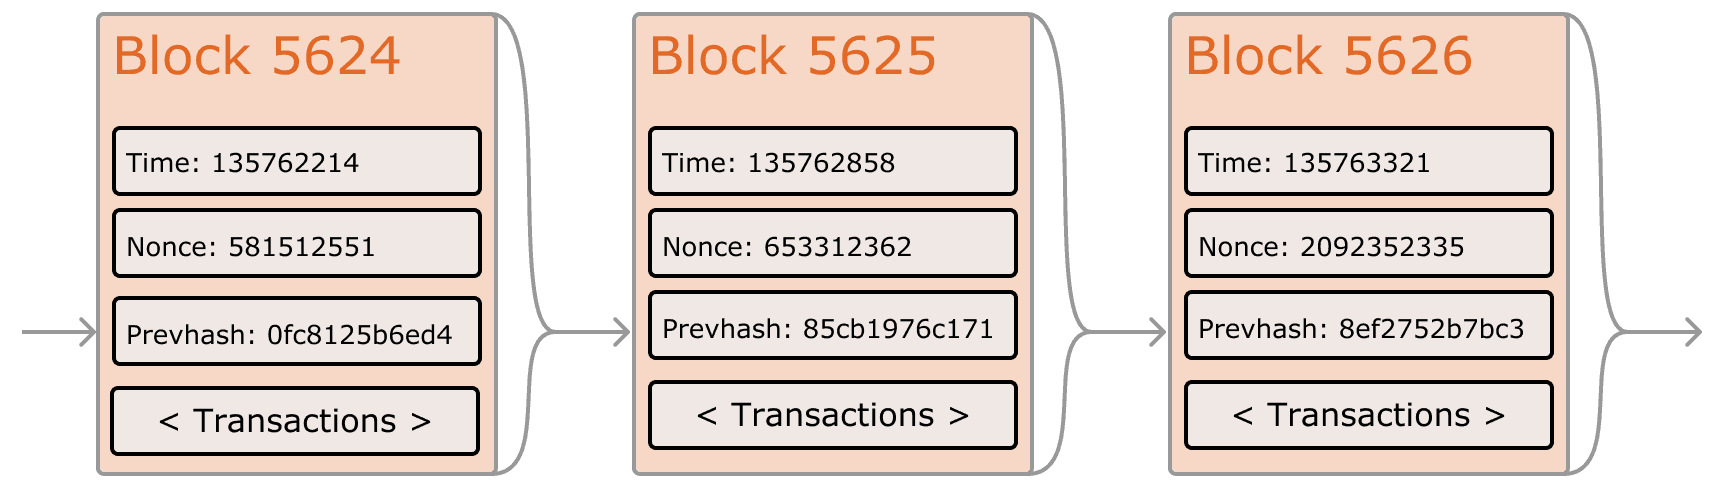
\includegraphics[width=\textwidth]{figures/ethereum-blocks.png}
        \caption{Ethereum blockchain structure.}
        \label{fig:ethereumBlockchainStructure}
    \end{figure}

    The Ethereum blockchain can be seen as a transaction-based, cryptographically secure state machine, that reads a series of inputs and, based on those inputs, transitions to a new state.
    Ethereum starts with a blank state called the “genesis state”.
    This genesis state transitions into a new state after executing a series of transactions.
    This new state represents the current state of the Ethereum blockchain, at any point in time.
    In other words, based on our analogy, blocks represent states and transactions represent state transitions.
    The data inside a block cannot be altered without changing all of its subsequent blocks.
    Changing all the subsequent blocks would require the consensus of the majority of the network.

    Every computer in the network must agree upon each new block and the chain as a whole.
    These computers are known as "nodes".
    Nodes act as an entry point to the blockchain and ensure everyone interacting with the blockchain has the same view on the data being recorded in the ledger.
    To accomplish this distributed agreement, blockchains make use of a consensus protocol.
    It is used to determine who is allowed to append the next block to the chain, and a random peer in the network has to be picked through it.
    Ethereum currently uses Proof-of-Work (PoW) as its consensus protocol.
    Proof-of-Stake (PoS) is another concensus protocol, for example.
    In order to append a new block to the blockchain, users have to generate a hash of the new block, which starts with a given number of zeros.
    Finding such a hash requires a lot of computing power.
    It acts as a “proof” that a node has done “work” by spending its computational resources.
    This process is known as mining and nodes which decide to participate in this process and try to create new blocks are known as miners.
    New blocks are then broadcast to the nodes in the network, checked and verified, thus updating the state of the blockchain for everyone.

    As participating nodes are allowed to propose new blocks simaltaneously and at nearly the same time, it can be the case that two or more blocks are proposed at once with a valid hash while referencing the same parent block.
    These competing branches that are created by these nodes are called “forks”.
    Blockchain forks pose a serious issue to Ethereum.
    They result in multiple concurrent states and make it difficult for the nodes to come to an agreement concerning which state should be the correct state.
    For example, if the states were to diverge, a user might own 100 coins on one chain, 200 on another, and 300 on another.
    Forks can happen intentionally or be deliberately orchestrated.
    To prevent multiple states and help determine which fork is the most valid one, Ethereum blockchain uses a technique known as the Greedy Heaviest Observed Subtree (GHOST) protocol.
    The GHOST protocol declares that of all the states, one must select the state that contains the most computation.
    One way to determine the heaviest state (computation-wise), is to look at the block number of the most recent block (i.e., leaf block) of a state, which amounts to the total number of blocks in the current state (not including the genesis block).
    The higher the block number, the longer the chain of that state and the greater the mining computation that must have gone into arriving at that current leaf block.
    This allows the blockchain nodes to agree on an accpeted version of the current state of the blockchain.
    Those blocks that are not included in the canonical chain are often referred to as orphans or uncle blocks.
    Unlike other blockchains, such as Bitcoin, Ethereum also adds uncle blocks to the aforementioned calculation to figure out the longest and computationally heaviest chain of blocks.
    This allows for the inclusion of more transactions and attributes a reward to the creators of uncle blocks as well as miners for declaring concurrent blocks as uncles and thereby keeping forked chains as short as possible.

    \begin{figure}
        \centering
        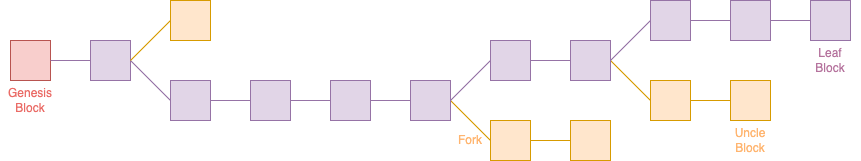
\includegraphics[width=\textwidth]{figures/uncle.png}
        \caption{An illustration of Ethereum's GHOST protocol.}
        \label{fig:uncle}
    \end{figure}

    \subsection{Ether}
        Ether is the native cryptocurrency of Ethereum.
        A cryptocurrency is a digital currency that is secured by means of cryptographic primitives.
        The purpose of ether is not only to allow users to exchange value between one another, but also to provide an economic incentive for users of its underlying platform to provide computational resources to the Ethereum network.
        Any network participant who sends a transactions must offer some amount of ether to the Ethereum network as a fee.
        This remuneration will be awarded to whoever gets to mine the block that includes the transaction, as a result of doing the work of verifying, executing, and broadcasting the transaction to the rest of the blockchain network.
        The amount of ether offered in such transaction as the corresponding fee, must correspond to the time and effort spent in executing the transaction.
        These costs prevent malicious participants from intentionally blocking up the network by requesting the execution of infinite computation or other resource-intensive actions, as these ill-intentioned participants must pay for the computation.

        Ethereum provides a metric system of denominations to describe different units of ether.
        Each denomination has its own unique name.
        Wei and Gwei are the most popular denominations.
        Wei is the smallest possible denomination of ether also known as the base unit, and as a result, many technical implementations base all their calculations in wei.
        Gwei (short for gigawei) is often used to describe costs related to “gas”.

    \subsection{Accounts}
        The global state of Ethereum is composed of many objects called “accounts”.
        They are able to interact with one another through so-called “messages”.
        Each account has a 20-byte address and a state associated with it.
        An address in Ethereum is a 160-bit identifier (a string of 42 hexadecimal characters) that is used to uniquely identify any account on the blockchain.
        There exist two different types of accounts (see Figure 2.4):
        
        \begin{itemize}
            \item \textbf{Externally Owned Accountss} (EOAs), which are controlled by private keys and have no code associated with them.
            \item \textbf{Contract Accounts} (CAs), which are controlled by their contract code and have code associated with them (i.e., smart contracts).
        \end{itemize}

        Both account types have the ability to receive, hold and send ether.
        EOAs can send messages to other EOAs and CAs by creating a transaction and signing it using their private key.
        The code that is associated with a CA, is executed whenever it receives a message from an EOA or a CA.
        The code allows a CA to perform various actions (e.g., write to storage, perform computations, etc.), which a EOA is not capable of.
        However, unlike EOAs, CAs cannot initiate new transactions on their own.
        Instead, CAs can only trigger messages in response to other messages that they have received from either an EOA or another CA.
        Thus, any actions that occurs on the Ethereum blockchain, are always set in motion by transactions that are triggered by EOAs.
        The account state consists of four fields, which are always present regardless of the type of account:

        \begin{itemize}
            \item \textbf{Nonce:} A number that acts as a simple counter which indicates the number of transactions sent from the account.
                This prevents the replaying of transactions and ensures that transactions are only processed once. If the account is an EOA, this number represents the number of transactions sent from the EOA's address. If the account is a CA, the nonce represents the number of contracts created by the CA.
            \item \textbf{Balance} The amount of cryptocurrency owned by this address in units of wei.
                Wei is the smallest subunit of ether (1 wei is equivalent to 10-18 ether).
            \item \textbf{Storage Root} A hash of the root node of the Merkle Patricia tree that encodes the storage contents of the account.
            This value is by default empty for both types of accounts and is solely updated for CAs whenever data is written to storage.
            \item \textbf{CodeHash} A hash of the bytecode associated with this account.
                For CAs, this represents a hash of the code that is stored on the blockchain. For EOAs, the this value is the hash of the empty string.
        \end{itemize}

        Creating an EOA has no cost as no data such as code, storage or balance is associated with the account at creation time.
        A CA on the other hand, has a cost because it uses the blockchain's storage to persist the contract code and data directly at creation time.

    \subsection{Transactions}
        Transactions are essentially cryptographically signed instructions from EOAs to update the state of the Ethereum blockchain.
        EOAs sign their transactions using their private key in order to cryptographically prove that the transaction could only have come from them and not from someone else.
        Two types of transactions exist: message calls and contract creations.
        The latter are transactions with an empty recipient field that result in creating new CAs (i.e., smart contracts). 
        The code, to be associated with the CA, is placed inside the data field of the transaction.
        Regardless of their type, all transactions contain the following fields:
            \begin{itemize}
                \item A count on the number of transactions sent by the sender. This number is incremented by one every time a transaction is sent by the sender.
                \item The amount of wei that the sender is willing to pay for each unit of gas that is used during the execution of the transaction.
                \item The maximum amount of gas units that the sender is willing to spent for the execution of this transaction.
                    This amount is set and paid upfront, before any computation is performed.
                \item The address of the recipient. If the recipient is an EOA, the transaction will transfer value, if the recipient is a CA, the transaction will transfer value as well as execute the contract's code.
                    A transaction with an empty recipient address is used to trigger the creation of a new CA.
                \item The amount of wei to be sent from the sender account to the recipient account.
                    Interestingly, this value may be used to set the starting balance of the newly created CA in a contract-creating transaction.
                \item These values represent the digital signature (R, S) which can be used to recover the public key (V).
                    These values identify the sender of the transaction and confirms that the sender has authorized the transaction.
                \item This field is only part of contract-creating transactions and consists of an unlimited length byte array that includes the code to be used during the initialization process and the code to be permanently associated with the newly created CA.
                \item This is an optional field that is only part of message calls and consists of a byte array of unlimited size that specifies the input data (e.g., , function name, function parameters) of the message call.
            \end{itemize}
            As previously mentioned, contract-creating transactions and message calls are always initiated by EOAs.
            However, this does not mean that CAs cannot communicate with other CAs.
            CAs can send messages or so-called “internal transactions” to other CAs.
            Internal transactions are similar to normal transactions, with the major difference being that they are not initiated by EOAs, but instead they are initiated by CAs.
            Moreover, internal transactions merely exist as virtual objects that, unlike transactions, are not persisted in the Ethereum blockchain and only exist at execution time.
            When a CA sends an internal transaction to another CA, the code that is associated with the recipient CA is executed.
            In contrast to normal transaction, internal transactions do not contain a gas limit by default.
            They are only limited by the gas limit that was determined by the normal transaction that triggered them.
            Thus, the gas limit that the EOA provides within its normal transaction, must be large enough to perform the execution of the normal transaction, including any sub-executions that occur as a result of that transaction, such as any internal transactions.
            If the execution of an internal transaction runs out of gas, then its execution will be will be reverted, along with any subsequent internal transactions triggered by the execution.
            However, the parent execution is not reverted.


    \subsection{Blocks}

        Blocks are batches of transactions with a reference to the hash of the previous block.
        This adds immutability and makes fraud noticeable, since a change in a transaction would invalidate all the previous blocks as all previous block hashes would change as well.
        Moreover, by grouping transactions into blocks, all network participants are given enough time to come to consensus, even in the case where hundreds of transactions are broadcast per second.
        The size of a block is usually bounded to a target size of 15 million gas units.
        However, the size of blocks will be increased or decreased depending on the demands of the network, up to a block limit of 30 million gas units (2x target block size).
        The total amount of gas spent by all transactions contained within the block must be less than the block gas limit.
        This is crucial as otherwise blocks could grow arbitrarily large and congest the blockchain.
        A block consists of a block header, a list of transactions, and a list of the block headers of the block's ommers.
        A block header consists of the following fields:

        \begin{itemize}
            \item \textbf{ParentHash}: A hash of the parent (previous) block's header (i.e., the pointer that links blocks together in a chain).
            \item \textbf{OmmersHash}: A hash of the current block's list of ommers. An ommer is a block whose parent is equal to one of the current block's parent's parent.
            \item \textbf{Beneficiary}: The account address that receives the fees for mining this block.
            \item \textbf{LogsBloom}: A Bloom filter (i.e., a data structure) that allows efficient querying of information contained in the logs.
            \item \textbf{Difficulty}: The effort required to mine this block.
            \item \textbf{Number}: The count of the current block. The block number of the genesis block starts at number zero and each subsequent block number is increased by one.
                The block number is often referred as the length of the blockchain in blocks.
            \item \textbf{GasLimit}: The current gas limit per block. This value represents the limit set on the overall gas consumption for this block.
            \item \textbf{GasUsed}: The sum of the total gas used by all transactions contained in this block. This value cannot surpass the GasLimit.
            \item \textbf{Timestamp}: The UNIX timestamp when the block was mined.
            \item \textbf{ExtraData}: Arbitrary data that can set by the miner. This data is limited to 32-byte and usually refers to the name of the miner or the client version that was used to mine the block.
            \item \textbf{MixHash}: A hash that, when combined with the nonce, proves that this block meets the difficulty of this block.
            \item \textbf{Nonce}: A value that, when combined with the MixHash, proves that this block has performed the required work.
            \item \textbf{StateRoot}: The hash of the root node of the Merkle Patricia trie that stores the state of all accounts (i.e., account balances, storage, code, and nonces).  The hash is calculated only after all transactions have been executed.
            \item \textbf{TransactionsRoot}: The hash of the root node of the Merkle Patricia trie that stores all transactions listed in this block.
            \item \textbf{ReceiptsRoot}: The hash of the root node of the Merkle Patricia trie that stores the receipts of all transactions listed in this block.
                Transaction receipts are generated after the execution of a transaction contain information such as logs or the actual gas that has been used during execution.

        \end{itemize}

        Block times are much lower in Ethereum (~15 seconds) than compared to those of other blockchains, such as Bitcoin (~10 minutes).
        The block time refers to the time that it takes to mine a new block.
        In Ethereum, the average block time is evaluated after each block.
        The expected block time is set as a constant at the protocol level and is used to protect the network's security when miners gain more computational power.
        The average block time is compared with the expected block time, and if the average block time is higher, then the difficulty contained in the block header is decreased.
        If the average block time is smaller, then the difficulty in the block header is increased.
        A smaller average block time enables faster transaction processing.
        However, shorter block times also means that miners will be more likely to find more competing block solutions.
        These competing blocks are often referred as ommers or uncles and are seen as “orphaned blocks”, hence, blocks that were mined but are not part of the canonical chain.
        The purpose of ommers is to incentivise miners to include orphaned blocks as a part of the canonical chain and thereby avoid forks.
        Miners are only allowed to include orphaned blocks that are not more than six block numbers away from the current block number.

    \subsection{Ethereum Virtual Machine}
        The Ethereum Virtual Machine (EVM) is a purely stack-based, register-less virtual machine that runs low-level bytecode and supports a Turing-complete set of instructions.
        For a simple analogy, you can think if it like the Java programming langauge that uses the Java Virtual Machine (JVM).
        It represents the execution model of a virtual state machine, defining how the states in the Ethereum blockchain are changed.
        Every instruction is represented by a one-byte opcode (e.g., 0x60 → PUSH1, e.g., 0x50 → POP, etc.).
        The instruction set consists of more than 140 different instructions ranging from basic operations such as arithmetic operations or control-flow operations to more specific ones, such as the modification of a contract's storage or the querying of properties related to the executing transaction (e.g., sender) or the current blockchain state (e.g., block number).
        The EVM uses a memory model that is specific to the execution of smart contracts and differs from the traditional von Neumann architecture (see Figure 2.7). Instead of organizing code and data in one large general-pu
        EVM is activated whenever a Smart contract on the Ethereum blockchain needs to be executed by receiving a message or transaction.
        Execution of a contract in EVM does not need any external resources from the network or file system, but there may exist some external calls to the functions of the other contracts in the blockchain.
        
        Instead of organizing code and data in one large general-purpose memory, the EVM follows the Harvard architecture by separating code and data into four different address spaces: (1) an immutable code address space, which contains the smart contract's bytecode, (2) a mutable but persistent storage address space that allows smart contracts to persist their data across executions, (3) a mutable but volatile memory address space that acts as a temporary data storage for smart contracts during execution, and finally (4) a stack address space that allows smart contracts to pass arguments to instructions at runtime.

        The EVM employs a gas mechanism that assigns a cost to the execution of an instruction.
        This mechanism prevents DoS attacks and ensures termination by solving the halting problem.
        When issuing a transaction, the sender has to specify a gas limit and a gas price.
        The gas price defines the amount of ether that the sender is willing to pay per unit of gas used.
        As the gas price is coupled to ether, developers are motivated to write efficient programs to keep transaction costs low and to avoid “infinite” loops.
        The base fee for executing a transaction starts at 21,000 gas units.
        The final execution costs are determined by multiplying the gas price with the gas used.
        The gas limit is specified in gas units and must be large enough to cover the amount of gas consumed by the instructions during a contract's execution, otherwise execution will terminate abnormally with an out-of-gas exception and its effects will be rolled back.
        The EVM also throws an exception when a jump destination is invalid, an instruction does not exist, or when there are not enough elements on the stack to perform an given operation.

        Instructions operate on a stack of 256-bit big-endian words.
        The stack is private to a single contract (but not to methods within the contract) and is almost free to use in terms of gas.
        The size of the stack is limited to 1,024 items.
        In addition to the stack, smart contracts can also store variables in memory.
        Memory is a random-access array of 256-bit words that is accessible only by the currently executing smart contract.
        Memory is always initialized with zeros and thus isolated from previous executions.
        Memory is also used to pass arguments across message calls.
        Figure 2.8 shows an example of an EVM message call.
        The CALL instruction first copies the arguments of the message call from memory into the input data of a new instance of the EVM.
        The control is then returned back to the message caller via the RETURN instruction and the return value that includes the result of the message call is placed into the memory of the caller.
        Besides stack and memory, the EVM also features storage.

        While stack and memory are volatile and may only hold values during execution, storage is persistent and part of the world state $\delta$.
        It is organized as a Patricia Merkle trie holding sets of key-value stores for each account.
        Storage is isolated from other smart contracts and is the only way for a smart contract to retain state across executions.
        While storage is theoretically unlimited, its use is expensive (compared to stack and memory) and should only be used to store small amounts of data.

\section{Smart Contracts}
    The concept of smart contracts has been first introduced by Nick Szabo in one of his works in 1997.~\cite{szabo1997formalizing}
    According to Szabo, smart contracts combine protocols, users' interfaces, and promises expressed via interfaces over public networks.
    Szabo described the notion of a system consisting of automatic, self-executing computer programs that would facilitate the enforcement of clauses contained in legal contracts and reduce mental and computational transaction costs, imposed by either
    principals, third parties or their tools.
    It took years for efficient trustless systems like blockchains such as Ethereum to develop and grow in order for them to utilize the concept of smart contracts in full, hence the 20-year delay between the ideation and real-world implementation of them.

    \subsection{Solidity}
        Solidity is an object-oriented programming language and it is currently the most prominent programming language for developing smart contracts in Ethereum.
        Its syntax resembles a mixture of C and JavaScript, but it comes with a variety of unique concepts that are specific to smart contracts and might be unfamiliar or confusing for new developers, such as the visibility of function modifiers: internal, external, pure, view, the function-wide scoping of variables, the emitting of events, or smart contract specific operations such as selfdestruct or revert.
        Similar to C, Solidity uses a function dispatch table to select what function to execute during runtime.
        The compiler does so by adding to the bytecode a function dispatcher that first loads the hash of the name of the function to be executed (the initial 4 bytes of the transaction input data Id) into the stack and then jumps to the function implementation that is associated with the hash (see Figure 2.9).
        Now, unlike C and JavaScript, the concept of “undefined” or “null” values does not exist in Solidity.
        Newly declared variables always have a default value depending on their type.
        For example, integers are always initialized with zero, whereas Boolean's are always initialized with False.
        Besides common variable types, such as int, bool, or string, Solidity also provides unique types such as mapping or address.
        The variable type mapping behaves similar to a dictionary in Python by mapping keys to values and therefore allowing an easy access to storage.
        The variable type address is meant to hold addresses of Ethereum accounts and has member function such as balance, send, transfer, call, etc.
        The member functions send, transfer, and call can be used to move ether from one address to another.
        All these functions make use of the EVM CALL instruction, with difference being the gas limit that can be used and the behavior on an error.
        
        Almost all variable types in Solidity are of type value, meaning that their value is copied when passed as an argument to a function.
        In contrast, the value of variable types of type reference, are not copied and therefore modified across function calls.
        Currently, variable types of type reference comprise mappings, arrays, and structs.
        Developers always have to explicitly state the data area where the type is stored when using a variable of type reference: memory (where its lifetime is limited to an external function call), or storage (where its lifetime is limited to the lifetime of the contract).
        In general, state variables are always stored in storage, function arguments are always stored in memory, and local variables of type value are stored in the stack.
        Moreover, Solidity suggests to be a statically typed language, i.e., the compiler expects type information for each variable to be made explicit.
        For instance, integers can be signed and unsigned, and of lengths between 8 and 256 bits in 8-bit steps denoted as uint8 or int128.
        This resembles integer types in C and may lead novice developers to assume that a uint8 will occupy 8 bits in memory, while an int128 occupies 128 bits.
        However, this assumption is wrong. Any integer type will be represented inside the EVM as 256-bit values in big endian order using two's-complement.
        That is, the integer type system of Solidity is not entirely consistent with that of the EVM, which can lead to programming errors.
        Explicit conversion between primitive types is possible, but the effects are not well documented.
        In fact, the documentation reads: Note that this may give you some unexpected behavior so be sure to test to ensure that the result is what you want.

        For example, explicitly casting a signed negative integer into an unsigned one will not result in the absolute value, but rather simply leave its bit-level representation intact.
        Interestingly, Solidity does not support floating points.
        However, similar to JavaScript, Solidity provides members such as length or push for arrays.

        Apart from variables, Solidity also provides units for ether and time (e.g., wei, days, etc.) as well as special keywords and functions which always exist in the global namespace and are mainly used as general-use utility functions or to provide information about the blockchain.
        Also mathematical and cryptographic functions are provided (e.g., addmod, ecrecover, etc.).
        For error handling, Solidity provides two convenience functions called assert and require, that can be used to check for a condition and to throw an exception if the condition is not met.
        Developers can interleave Solidity statements with inline assembly in a language called Yul, which is close to the one of the EVM.
        This gives more fine-grained control and bypasses optimizations imposed by the compiler.
        An inline assembly block is marked via the keyword assembly.
        The inline assembly code can access local Solidity variables, but different inline assembly blocks cannot call functions or access variables defined in a different inline assembly block.

    \subsection{Bytecode}
        Ethereum bytecode consists of a sequence of bytes that is interpreted by the EVM.
        Each byte either encodes an instruction or data.
        Figure 2.10 depicts the anatomy of Ethereum bytecode.
        Ethereum bytecode consists of two main parts: deployment bytecode and deployed bytecode.
        Deployment bytecode includes the deployment logic of the smart contract.
        This logic is responsible for initializing state variables and reading constructor arguments appended at the end of the Ethereum bytecode.
        It is also in charge of extracting the deployed bytecode from the Ethereum bytecode and copying it to persistent storage.
        This is achieved via the CODECOPY and RETURN instructions.
        Starting from a given offset and for a given size, the CODECOPY instruction first copies the code running in the current environment to memory.
        Afterwards, the RETURN instruction returns the code that has been copied into memory to the EVM.
        As a result, the EVM creates a new contract by generating a new 160-bit address and persisting the returned code with this new address.
        The deployed bytecode contains the runtime logic (i.e., runtime bytecode) and optional metadata.
        The runtime bytecode is the logic that is executed whenever a transaction is sent to a smart contract.
        Some compilers, such as the Solidity compiler, also append some metadata (e.g., compiler version) to the end of the runtime bytecode.

    \subsection{Vulnerabilities}
        Atzei et al.~\cite{atzei2017survey} were the first to publish a survey of smart contract vulnerabilities and their corresponding attacks.
        However, their survey goes back to 2016.
        Since then, several new vulnerabilities and attacks have emerged (e.g., Parity wallet hacks, integer overflows, etc.).
        In 2018, the NCC Group released their own inititative of ranking smart contract vulnerabilities, namely, the Decentralized Application Security Project (DASP).~\cite{dasp}
        It is an open and collaborative project to join efforts in discovering and documenting smart contract vulnerabilities within the security community.
        The idea is similar to the well known Open Web Application Security Project (OWASP).
        However, neither the ranking nor the list of vulnerabilities has been updated since its first release in 2018.
        Another initiative to document well-known attacks is the one presented by ConsenSys, called the Smart Contract Weakness Classification Registry (or simply SWC Registry).~\cite{swcregistry}
        It has been released with the goal to provide a common way to report and classify security issues in smart contracts.
        It loosely resembles the terminology and structure used in the Common Weakness Enumeration (CWE) project.
        Unfortunately, their list only contains a handful of vulnerabilities.
        At the time of writing, it includes 37 entries.
        Each entry consists of an identifier (SWC-ID), a weakness title, a CWE parent, and a list of related code samples.
        In 2019, Chen et al. ~\cite{chen2020survey} presented a survey of vulnerabilities, attacks, and defenses for the Ethereum blockchain.

        We provide in the following a detailed explanation of some of the more prominent smart contract vulnerabilities according to the above-mentioned DASP collection of vulnerabilities:

        \paragraph{Re-entrancy}
            A typical flaw in smart contracts are re-entrant calls.
            Re-entrancy may occur whenever a contract sends a value to or calls a function from another contract, and the called contract has enough gas to call back the original contract.
            As a result, the called contract re-enters the original contract.
            Therefore, the original contract must guarantee that its state is always correct, independent of re-entrant calls.
            Otherwise, a malicious contract can take advantage of an incorrect intermediate state to steal funds.
            The 2016 DAO hack remains the most famous example of a reentrancy attack not only because an unknown attacker managed to steal funds worth 50M USD [47], but also because it led to a hard fork of the Ethereum blockchain [164].
            A way to protect against reentrancy is to use the Solidity methods send or transfer rather than call.
            The aforementioned methods limit the amount of gas to 2,300 units, which makes it impossible for the called contract to modify the state or make any function calls.
            However, this only protects the sending of value.

        \paragraph{Access Control}
            A typical design pattern in smart contracts is to assign an address as the owner of the smart contract [107].
            This address has then privileged access to functions that can either update sensible variables, transfer funds, or destroy the entire contract.
            Unfortunately, this also means that faulty implementations of access control can lead to devastating consequences. One example of a flawed access control implementation is the use of Solidity's tx.origin to check whether the current address is authenticated to perform a sensible function call such as the withdrawal of funds.
            However, tx.origin does not represent the currently calling address, but the very first address that initiated the transaction.
            Remember that within a transaction, contracts can call other contracts, and therefore the calling address can be a different one at runtime.
            An attacker can perform a man-in-the-middle attack by first convincing a victim to send a transaction to the attacker's contract, which then performs within the same transaction a message call to the victim's wallet.
            If the wallet checks for the transaction origin to authenticate users, then the attacker will be authenticated as the victim and might be able to steal the funds.
            Developers should, therefore, rely on the msg.sender property to authenticate user accounts.

        \paragraph{Bad Randomness}
            Randomness is hard to achieve in general. In Ethereum it is even harder, since smart contracts are executed in a deterministic way.
            However, games and lotteries sometimes require non-deterministic values. Therefore, a variety of smart contracts rely on “unpredictable” information originating from yet unmined blocks, such as blockhash or number. They most often use this information as a seed to generate pseudo-random numbers. However, because the sources of randomness are predictable, malicious users can brute force the values of blocks before they have been mined.
            The Run [43] and SmartBillions [69] are famous examples of smart contract lotteries using block information for generating random numbers.
            In October 2017, an attacker was able to exploit the predictability of block information and steal 400 ether from the SmartBillions contract [84].

        \paragraph{Frontrunning}
            Users observing the network can see and react to transactions before they are mined. Miners typically order transactions based on their gas prices.
            This results in gas price wars between users in the network.
            Frontrunning is therefore also known as transaction order dependence (TOD).
            A decentralized exchange is a perfect example on how this can be exploited. An attacker observes a transaction containing a large buy order and quickly broadcasts its own transaction containing a buy order with a larger gas price in order to be executed before the observed buy order.
            A few other cases related to frontrunning have been studied by Eskandari et al.~\cite{eskandari2019sok}
            Common mitigations against frontrunning include the use of commit and reveal schemes or the specification of a minimum or maximum acceptable price range on a trade, thereby limiting price slippage.
        
        \paragraph{Time Manipulation}
            Sometimes smart contracts need to rely on the current time to either be able to accomplish their defined task, such as locking a token sale, or unlocking funds at a specific time in a game.
            In Solidity, the current timestamp is retrieved via \texttt{block.timestamp} or \texttt{now}.
            However, this value can be set by miners and can be manipulated.
            If a miner holds enough value inside a smart contract, then the miner could gain an advantage by choosing a suitable timestamp for a block that he or she mines.
            Smart contracts should, therefore, avoid relying on timestamps originating from blocks.
            Atzei et al. stated that the ponzi smart contract GovernMental is vulnerable to a timestamp manipulation attack~\cite{atzei2017survey}.
            However, there is no reported incident of such an attack in the wild.
        
        \paragraph{Short Address}
            Short address attacks are a side-effect of the EVM itself accepting incorrectly padded arguments. 
            Function arguments are typically encoded as 32-byte chunks of data within the input field of an Ethereum transaction.
            However, if the length of an encoded argument is shorter than 32 bytes, then EVM will auto-pad extra zeros to the end of the argument so that it always has a length of 32 bytes, no matter the size of the original encoding.
            Attackers can exploit this vulnerability by generating specially-crafted addresses that end with trailing zeros.
            The EVM does not check the validity of addresses, and the only way to prevent this attack is to check the length of a transaction's input at smart contract scope using \texttt{msg.data}.

\chapter{Automated Vulnerability Analysis of Smart Contracts on Ethereum} 
\label{ch:Slither-simil}

% \textit{
% This chapter is adapted from work supervised by Jeremy Clark and Mohammad Mannan, and is accepted for publication at the 2022 Workshop on Trusted Smart Contracts (WTSC) co-located with Financial Cryptography and Data Security (FC).
% }

\section{Introductory Remarks}
Smart contracts, the universal and vital programs that are deployed on blockchains, have gained increasing attention with the rapid development of blockchains.
For example, more than 10 million smart contracts have been deployed on the Ethereum Mainnet.

smart contract is an event-driven, state-based program that is written in high level languages such as Solidity.
Smart contracts have been widely used in many business domains to enable efficient and trustful transactions.

Unlike general programs, the development of smart contracts requires special effort due to their unique characteristics.
First, smart contracts are more bug intolerant compared with general programs.
“Code is law”, a smart contract can not be modified once it has been released. 
This is because transactions of a smart contract always involve cryptocurrencies which are worthy of millions of dollars (e.g. The DAO). 
A bug in a smart contract may lead to a substantial loss.
Therefore, ensuring the correctness of contracts before releasing is critical.
 This requires us to reuse experience of developed contracts in the past when developing new contracts.
Program mining for smart contracts such as summarization, checking, and code search can greatly facilitate the development and maintenance of smart contracts.
The conventional statistical analysis tools for detecting weaknesses in smart contracts purely rely on manually defined patterns, which are likely to be error-prone and can cause them to fail in complex situations.
As a result, expert attackers can easily exploit these manual checking patterns.
To minimize the risk of the attackers, machine learning powered systems provide more secure solutions relative to hard-coded static checking tools.

Throughout our research, we noticed the future direction of the literature on smart contract vulnerability detection, and our goal is to provide guidance for new developments in this field.
In order to set the ground for further development of ML method on smart contract vulnerability detection, in this survey paper, we reviewed many ML-driven intelligent detection mechanism on the following databases: Google Scholar, Engineering Village, Springer, Web of Science, Academic Search Premier, and Scholars Portal Journal.
We provided our insights on limitations and advancement of ML-driven solutions.


\section{Existing Analysis Tools}

Classic software testing technologies applied towards smart contract security analysis can be diivied into three categories; In the following, we will go over the tools proposed from the perspective of the technology they employ to tackle the smart contract security problem:

\paragraph{Static Analysis}
Static analysis is the method of analyzing a computer program of a program without running it, which can be performed at both source code and bytecode level.
Tools that employ the method of static analysis are able to scan the entirety of a code base base but also produce much false positives in the results of their scans.
SolidityCheck~\cite{soliditycheck} retrieves each function at the source code level and checks the piece that matches the pre-defined vulnerability patterns.
Normally, other tools will first obtain binary bytecode, and then use it to construct a custom intermediate representation, which have a series of forms, like SSA used in Slither~\cite{slither}, Datalog used in Securify~\cite{securify} and MadMax~\cite{madmax}, XML parsing tree used in SmartCheck~\cite{smartcheck} and XCFG used in ClairvOyance~\cite{ClairvOyance}.
Based on this representation, vulnerability pattern definition and matching are performed to screen out suspected code snippets.
As a static analysis method based on mathematical proof, formal verification is also widely used to verify the logical integrity of smart contracts, such as EtherTrust~\cite{etehrTrust}, VeriSmart~\cite{verismart} and Zeus~\cite{kalra2018zeus}.

\paragraph{Dynamic Analysis}
Fuzzing is a method of discovering software failures by constructing unexpected input data and monitoring the abnormal results of the target program during execution.
It allows developers to ensure a uniform standard of quality through prepared tests, but does not narrow down the causes of detected bugs.
When applied to smart contracts, a fuzzing engine will first try to generate initial seeds to form executable transactions.
With reference to the feedback of test results, it will dynamically adjust the generated data to explore as much smart contract state space as possible.
Finally, it will analyze the status of each transaction based on the finite state machine to detect whether there is an attackable threat.
ContractFuzzer~\cite{contractfuzzer} is the first to apply fuzz testing to smart contracts. Later, other researchers start to study improvements to different parts of fuzzing.
ReGuard~\cite{liu2018reguard} and Harvey~\cite{wustholz2020harvey} are dedicated to generating diverse inputs and transactions that are more likely to reveal vulnerabilities, ILF~\cite{he2019learning} and sFuzz~\cite{nguyen2020sfuzz} target at designing more effective generation or mutation strategy.

\paragraph{Symbolic Execution}
When using symbolic execution to analyze a program, it will use symbolic values as input instead of the specific values during the execution.
When a fork is reached, the analyzer will collect the corresponding path constraints, and then use a constraint solver to obtain specific values that can trigger each branch.
Symbolic execution can simultaneously explore multiple paths that the program can take under different inputs, but it also faces unavoidable problems such as path explosion.
In most cases, the symbolic executor will first build a control flow graph based on Ethereum bytecode, then design corresponding constraints based on the characteristics of smart contract vulnerabilities, and finally use the constraint solver to generate satisfying test cases; for example, Oyente~\cite{oyente}, Mythril~\cite{mythril}.
In recent years, there has been continuous research to optimize the process of symbolic execution.
Manticore~\cite{mossberg2019manticore} adds the support of exotic execution environments, DefectChecker~\cite{chen2021defectchecker} extracts defect related features to help improve efficiency, sCompile~\cite{chang2019scompile} identifies critical paths which involve monetary transaction and VerX~\cite{permenev2020verx} focuses on verifying effectively external callback free contracts.

\section{Deep Learning in Smart Contracts} \label{sec:dl-models}

In this section, we will go over some of the literature focusing their efforts on replacing the existing tools' capabilities explained in the previous section with amchine learning-based techniques. Afterwards, we will go over our own developed tool, Slither-simil.

There have been a lot of efforts focused towards utilizing ML based techniques in the field of vulnerability mitigation with a specific focus on the programming language Solidity and its lower level representations.

In 2018, Goswami et al. mentioned that while existing symbolic tools (e.g., Oyente) for analyzing vulnerabilities have proven to be efficient, their execution time increases significantly with depth of invocations in a smart contract ~\cite{grech2019gigahorse}.
They proposed an LSTM neural network model to detect vulnerabilities in ERC-20 smart contracts in an effort to produce a less time consuming and efficient alternative to symbolic analysis tools.
The preprocessing steps followed in this paper were very similar to the methods used by ~\cite{madmax}.
The model was trained and tested on a dataset of 165,652 ERC-20 smart contracts, which consisted of bytecode data labeled by Maian and Mythril (statistical code analysis tools).
The proposed model achieved 93.26\% accuracy, 92\% recall and an F1 score of 93\% on the testing set.
Further they have compared the time performance of their model to those of the symbolic analysis tools Maian and Mythril (static analysis tools).
While their proposed model had a runtime of 15 seconds on a testing set of 5,000 random tokens, Maian and Mythril took 32,476 and 9,475 seconds respectively.
These results indicate the same type of improvement achieved over symbolic analysis tools as in ~\cite{grech2019gigahorse}.

In 2018, Liao et al. have adopted a sequence learning approach to detect smart contract security threats ~\cite{madmax}.
Smart contract data was obtained from the Google Big Query Ethereum blockchain dataset.
Ultimately, an LSTM model was trained on 620,000 contracts from this source. Once again, the derived opcodes from the contracts were represented as one-hot vectors.
As this type of representation results in highly sparse and uninformative features, these vectors were transformed into code vectors using embedding algorithms, resulting in lower dimensionality and a higher capability of capturing potential relationship between sequences.
As another preprocessing step, they have compared the statistical properties of the opcode lengths of contracts that were identified as vulnerable and safe.
Having observed that the properties of the two categories differ significantly, they have limited the input data to the LSTM to only include contracts that had a maximum opcode length of 1600, as a design choice.
Further, the distribution of the dataset (labeled by MAIAN) was realized to be imbalanced with non-vulnerable instances making up 99.03\% of the dataset.
Therefore, all vulnerable contracts were grouped together and oversampled to achieve a balanced distribution in the training set using the Synthetic Minority Oversampling Technique (SMOTE).
The results indicated the superiority of a sequential learning approach over symbolic analysis tools.
The model achieved a vulnerability detection accuracy of 99.57\% and F1 score of 86.04\%.

In 2019, SoliAudit model was proposed to enhance the vulnerability detection of smart contracts ~\cite{etehrTrust}.
Smart contract source code in Solidity is converted into an opcode sequence to preserve the structure of executions.
Each contract goes through both a dynamic fuzzer and a vulnerability analyzer.
The vulnerability analyzer consists of a static machine learning classifier, which detects vulnerable classes, whereas the fuzzer (this term was introduced in an earlier paper) will parse the Application Binary Interface (ABI) of a smart contract to extract its declared function descriptions, data types of their arguments and their signatures.
It will then return the smart contract inputs and functions that are identified as vulnerable.
The idea of a smart contract fuzzer was introduced by the authors of ~\cite{etehrTrust}.
Vulnerability analyzer used a set of labels (13 vulnerabilities) determined by analysis tools such as Oyente and Remix.
Before training the opcode sequence data using these labels, two types of feature extraction methods were tested. These were namely, n-gram with tf-idf and word2vec.
The experiments were carried out by applying the former method together with algorithms such as Logistic Regression, Support Vector Machine, K-Nearest Neighbor, Decision Trees, Random Forests and Gradient Boosting.
The output from the latter (word2vec) was a matrix and a Convolutional Neural Network (CNN) was preferred to train it as it considers the inner structure of the matrix.
However, this combination of feature extraction and training did not yield good results.
The best results for the classification of vulnerabilities were obtained using Logistic Regression with an accuracy of 97.3\% and F1 score of 90.4\%.

In 2020, Xing et al. ~\cite{hu2021comprehensive} developed a new feature extraction method called slicing matrix, which consists of segmenting the opcode sequences derived from smart contract bytecodes to extract opcode features from each one individually.
The purpose of this segmentation is to separate useful and useless opcodes.
The extracted opcode features are then combined to form the slice matrix.
To carry out a comparative analysis, three models were created.
These were namely Neural Network Based on opcode Feature (NNBOOF), Convolution Neural Network Based on Slice Matrix (CNNBOSM), Random Forest Based on opcode Feature (RFBOOF) ~\cite{hu2021comprehensive}.
These three models were each tested on three different vulnerability classification tasks: greedy contract vulnerability, arithmetic overflow/underflow vulnerability and short address vulnerability.
While RFBOOF achieved the best results in all three cases based on precision, recall and F1 evaluation metrics, CNNBOSM performed slightly better than NNBOOF in general.
The authors mention that the slice matrix feature need further exploring.

In 2020, In N. Lesimple et al.'s paper ~\cite{day2019ethereum}, the authors study the effect of deep learning models when used to identify vulnerabilities in Smart Contracts.
It specifically highlights the vulnerabilities relating to Domain Specific Languages (DSL), which is defined as a language engineered to work solely on a single program.
This is highly relevant for blockchain, as Solidity was specifically designed for Ethereum, and therefore is a DSL.
The authors then identify some common vulnerabilities in traditional smart contract code, and examine issues with traditional vulnerability checking techniques.
Of these, one of the most important issues with traditional techniques is that the subset of bugs found are due to the strict predefined inputs that are used.
The paper proposes that, through the use of Deep Learning, the input can be varied significantly to identify faults that the predefined static tests would otherwise not.
The authors then propose a novel approach, which analysis the line level code and trains a Deep Learning Neural Network to understand the control paths and data transformations occurring in the code ~\cite{day2019ethereum}.
As an input to the model, to allow for the model to understand the code on a line level, the authors used an Abstract Syntax Tree (AST) structure, which relates variables to one another, marking their dependencies and transformations throughout the code.
The author analyzed several Natural Language Processing techniques, and Recurrent Neural Networks, and eventually landed on using an LSTM network to train their model.
They found that LSTM's outperformed most RNN models, and due to the vast variety in code syntax, the NLP techniques were unable to interpret many situations, since the code and inputs were inconsistently structured.
Their results were quite accurate, but it is important to note that the results were tested against results from a traditional model that they were actually attempting to replace.
If this paper could acquire a test set of vulnerabilities that were not acquired through the use of a traditional method, the results would be more poignant.

In 2021, Liu Z. et al. proposed a combining GNN and expert knowledge based machine learning model for detecting various smart contract vulnerabilities ~\cite{hwang2020gap}.
A graph neural network (GNN) is a deep learning method, where the principle is to perform inference on data described by graphs.
In computer science, a graph is a data structure consisting of two components: nodes (vertices) and edges. Researches have proven that written programs can be converted to symbolic graph representation, without disrupting semantic relationship between programming elements.
Thus, smart contract codes can be represented as contract graphs.
In the experiment, ESC (Ethereum Smart Contracts) and VSC (VNT chain Smart Contracts) real world datasets (containing 320,000 contracts), where ESC was used to evaluate timestamp dependence vulnerabilities, while contracts from VSC is utilized for infinite loop vulnerabilities.
The proposed model consists of two different parallel processes (Security pattern extraction and contract graph extraction) at the beginning, and the combining layer merged patterns in each section to find vulnerabilities, as shown in figure 3.
First, a feed-forward neural network generates the pattern feature for extracting security patterns from the contract's source code.
They have used an opensourced tool to extract the expert patterns from smart contract functions.
The second process (message propagation phase) is to create a GNN to achieve a contract graph.
Inside the GNN model, nodes were the program elements (i.e., function), where edges represented the flow (i.e., next function to be executed) of each program elements.
Later, unwanted nodes and edges are removed based on a node elimination strategy.
As a preprocessing method, the authors casted rich control and data flow semantics of the source code into a contract graph.
After this step, they designed a node elimination stage to highlight critical nodes by normalizing the graph.
These two parallel processes were combined using vulnerability detection phase, where both extracted features are combined convolution and full-connected layer.
In experiment, the proposed model is compared with non-ML-based security detection algorithms, namely Oyente, Myhrill, Smartcheck, Securify, and Slither.
Each algorithm and the proposed model performed a search of several vulnerabilities (re-entrancy, timestamp dependence, and infinite loop vulnerabilities) of each function in the source code.
aThe proposed algorithms (CGE) achieved 89\% accuracy on finding re-entrancy and timestamp dependence type of vulnerabilities, and 83\% accuracy on detecting infinite loop vulnerability ~\cite{hwang2020gap}.

In 2021, Eth2Vec model is proposed to deficiency in current vulnerability detection tools when a code is rewritten. In programming languages, a code rewrite is reimplementing a source code's functionality without reusing it.
When the smart contract codes are rewritten, detecting vulnerabilities become harder.
The authors first converted each smart contract source code into EVM bytecodes.
From the bytecode, the authors extracted only valuable information (i.e., function id, list of callee functions etc.) for vulnerability detection.
As the last process, a neural network structure is used to catch any vulnerabilities in the source code.
After testing the proposed model on 500 contracts, the Eth2Vec model was able to detect vulnerabilities with a 77\% precision even though the contracts are rewritten.

In 2021, O. Lutz et al.~\cite{dolan2016lava} introduce yet another method of detecting vulnerabilities within smart contracts.
The authors propose a solution entitled ESCORT, wherein they use a Deep Neural Network model to learn the semantics of the input smart contract, and learn specific vulnerability types based on the found semantics.
The goal of the ESCORT model is to overcome the scalability and generalization limitations of traditional non-DNN models.
Experimental results of this paper yielded an F1 accuracy score of 9\% on six found vulnerability types, with a detection time of 0.02 seconds per contract.
With such quick detection times, scalability is more easily achieved, satisfying one of the author's goals.
Then, through the use of transfer learning, the ESCORT model slightly overcomes the issues found in other papers, such as Y. Xu or N. Lesimple's models~\cite{grech2019gigahorse}, where newfound vulnerabilities can be realized by the model.
Unfortunately, it is rather difficult to obtain interpretability from such models, and though new vulnerabilities may be found, understanding their cause remains to be exceedingly difficult.

In 2021, Sun et al. have attempted to detect the following vulnerabilities: re-entrancy, arithmetic issues (integer overflow/underflow) and timestamp dependence using machine learning ~\cite{grech2019gigahorse}.
As a common prerequisite step, some stackoperating instructions were truncated into more general forms (e.g., SWAP1, SWAP2, ..., SWAPn. → SWAPx) to account for variations in instructions among different compilers.
Following this, opcodes were separated into 9 categories based on their functions, as a label normalization step.
As in ~\cite{etehrTrust} a word2vec transformation of the opcode sequences, preceding the convolutional layers, was performed.
In addition to the pooling and softmax layers that commonly follow convolutional layers, this paper introduces an additional self-attention layer.
The purpose of the self-attention layer is to create a connection between adjacent words in the obtained feature matrix since one-hot encoders that were used to encode each opcode instruction are just mere representatives and do not capture any functional similarity between them ~\cite{grech2019gigahorse}.
As a result, the word embedding process has been enhanced through the use of self-attention.
When compared to the vulnerability detection performance of ~\cite{etehrTrust}, they have both used a CNN but ~\cite{etehrTrust} used a word2vec embedding whereas this paper employed an attention mechanism, which is the likely reason that they obtained better results.
obtained better results. The main improvement of the created model over the existing static analyzers such as Oyente and Mythril is that it can achieve comparable performance in much less time.

In 2019, Pouyan et al. employed popular supervised ML models to classify vulnerabilities in 1000 smart contracts [7].
The dataset was built collecting 1,013 smart contracts from Etherscan, where 80\% was used for training and the remaining was used for testing purposes.
In order to label each contract based on its source code's character, they used three different feature extraction techniques: abstract syntax tree (AST), control flow graph (CFG), and Static code analysis.
The extracted features were grouped in two: features that represents execution path (e.g., function calls) and were directly added to the control flow graph. The authors used Slither and Mythrill to assign labels to each contract. 36 types of vulnerabilities were used to label each contract in test and train set. Vulnerability detection process was performed with common ML models: Support Vector Machine (SVM), Neural Network (NN), Random Forest (RF), and Decision Tree (DT). After training each model with training set, they were ranked based on the following evaluation metrics: accuracy, recall, F1, and precision. Due to the results, ML models were be able to identify 16 vulnerabilities among 36 with high performance. It was found that some specific ML models were more successful in finding certain vulnerabilities. For example, SVM model was successful of finding integer outflow, while NN achieved superior results detecting re-entrancy vulnerability. Due to the article’s summary, it was proven that extracted features of smart contracts can be passed to any popular ML model for vulnerability detection. Also, it is important to note that static code analyzers' execution time (7,311 seconds) was drastically slower than any ML model (0.32 seconds) [7]

In 2021, a vulnerability and transaction behaviour-based detection is proposed ~\cite{contractfuzzer}
 In this work, the authors built a model that correlates malicious activities, and the vulnerabilities present in smart contracts.
 In respect to strength of the correlation unsupervised ML models (K-means and HDBSCAN) assign a severity score to each smart contract.
 The model was trained to detect suspects among benign smart contracts. The aim of the research was to test their hypothesis, which was “the transaction behavior is a more critical factor in identifying malicious smart contracts than vulnerabilities in the smart contract.” Thus, they brought a different perspective to the literature of smart contracts vulnerability detection.

In 2021, Y. Xu et al.'s paper introduced two novel smart contract vulnerability detecting approach using both a KNearest Neighbors (KNN) model and a Stochastic Gradient Descent (SGD) model~\cite{slither}.
Identifying some common vulnerabilities identified by traditional methods today, they attempt to use each of the machine learning models to identify eight of the most prominently recognized traditional vulnerability types: re-entrancy, arithmetic, access control, denial of service, unchecked low level calls, bad randomness, front running, and denial of service.
As with N.Lesimple's paper~\cite{he2019learning}, the input to their model uses an AST structure, allowing the model to gather line by line information about the smart contract code.
The labels for the vulnerabilities were identified using traditional methods.
The paper notes high accuracy, precision and recall, for four of the eight vulnerabilities.
The other four did not have enough samples in the dataset, and the corresponding results were recognized as inconclusive. As with the N. Lesimple paper, the test set was created from results from using traditional methods, indicating that the authors were unable to illustrate how the KNN model differed from traditional techniques.

In 2021, ContractWard model is proposed as a faster alternative for Oyente~\cite{oyente}.
The dataset consisted of 49502 smart contracts, where each of them contained six possible vulnerabilities: integer overflow/underflow, transaction ordering dependency, call stack depth attack, timestamp dependency, and re-entrancy vulnerability.
Each contract's source code is converted to opcodes.
On average, a smart contract contains 4364 opcode elements with 100 types of opcodes in total.
After the simplification process, there were only 50 opcode types left.
Due to that reason, the authors wrapped opcodes with similar functionalities in a same category, and ultimately simplified features in the dataset.
Later, they used n-gram technique (sliding window of binary-byte size) to track relations of each opcodes, since they assume that the operations have higher relation with its neighbors.
Oyente was used to assign multi label to each contract.
After the labeling process, the researchers encountered class-imbalance problem, due to rarity of some vulnerabilities.
They employed synthetic minority oversampling technique to extend the number of minority class.
The training process adopted 5 candidate ML models: eXtreme Gradient Boosting (XGBoost), Adaptive Boosting (AdaBoost), Random Forest (RF), Support Vector Machine (SVM), and k-Nearest Neighbour (KNN).
In evolution stage, Micro-F1 and MicroF1 (variations of F1 metric) is utilized to rank the predictors.
The XGBoost model showed a robust performance by achieving over 96\% F1, Micro-F1, and Macro-F1score.

\section{Slither-simil}
Our efforts with regard to automating smart contract security assessments was to work on an addition to an already prominent static analysis tool, to better help developers and researchers in their process of auditing dmart contracts.

Trail of Bits, a prominent blockchain security firm has manually curated a wealth of data—years of security assessment reports—and we decided to explore how to use this data to make the smart contract auditing process more efficient with an addition to Slither -a static analysis tool-named Slither-simil.

Based on accumulated knowledge embedded in previous audits, we set out to detect similar vulnerable code snippets in new clients' codebases. Specifically, we explored machine learning (ML) approaches to automatically improve on the performance of Slither, our static analyzer for Solidity, and make life a bit easier for both auditors and clients.

Currently, human auditors with expert knowledge of Solidity and its security nuances scan and assess Solidity source code to discover vulnerabilities and potential threats at different granularity levels.
In our experiment, we explored how much we could automate security assessments to:
\begin{enumerate}
  \item Minimize the risk of recurring human error, i.e., the chance of overlooking known, recorded vulnerabilities.
  \item Help auditors sift through potential vulnerabilities faster and more easily while decreasing the rate of false positives.
\end{enumerate}

Slither-simil~\cite{slithersimil}, the statistical addition to Slither, is a code similarity measurement tool that uses state-of-the-art machine learning to detect similar Solidity functions.
When it began as an experiment last year under the codename crytic-pred, it was used to vectorize Solidity source code snippets and measure the similarity between them.
This year, we took it to the next level and applying it directly to vulnerable code.

Slither-simil currently uses its own representation of Solidity code, SlithIR (Slither Intermediate Representation), to encode Solidity snippets at the granularity level of functions.
We thought function-level analysis was a good place to start our research since it's not too coarse (like the file level) and not too detailed (like the statement or line level).

SlithIR is the hybrid intermediate representation used in Slither to represent Solidity code. Each node of the control flow graph can contain up to a single Solidity expression, which is converted to a set of SlithIR instructions.
This representation makes implementing analyses easier, without losing the critical semantic information contained in the Solidity source code.

SlithIR uses fewer than 40 instructions. It has no internal control flow representation and relies on Slither's control-flow graph structure (SlithIR code is associated with each node in the graph).
The complete descriptions is available at~\cite{slithir}.

\begin{figure}
  \centering
  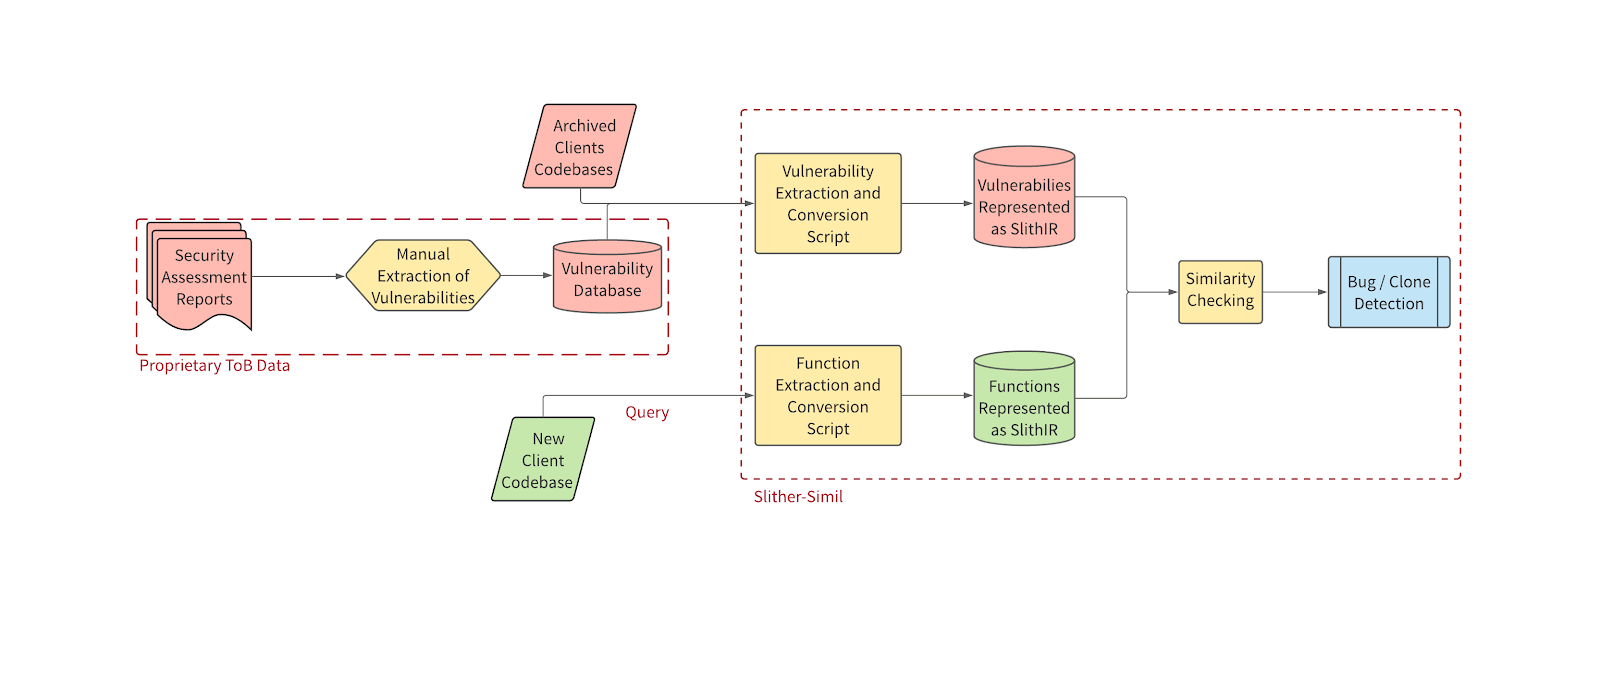
\includegraphics[width=\textwidth]{figures/slitherS.png}
  \caption{A high-level view of the process workflow of Slither-simil.}
  \label{fig:slithersimilhighlevel}
\end{figure}

In the process workflow of Slither-simil, we first manually collected vulnerabilities from the previous archived security assessments and transferred them to a vulnerability database.
Note that these are the vulnerabilities auditors had to find with no automation.

In the process workflow of Slither-simil, we first manually collected vulnerabilities from the previous archived security assessments and transferred them to a vulnerability database.
Note that these are the vulnerabilities auditors had to find with no automation.

After that, we compiled previous clients' codebases and matched the functions they contained with our vulnerability database via an automated function extraction and normalization script.
By the end of this process, our vulnerabilities were normalized SlithIR tokens as input to our ML system.

Here's how we used Slither to transform a Solidity function to the intermediate representation SlithIR, then further tokenized and normalized it to be an input to Slither-simil:

\begin{lstlisting}[float,caption= complete Solidity function from the contract TurtleToken.sol., escapechar=\%, language=Solidity, label=lst:solidity-bug]
  function transferFrom(address _from, address _to, uint256 _value) public returns (bool success) {
        require(_value <= allowance[_from][msg.sender]);     // Check allowance
        allowance[_from][msg.sender] -= _value;
        _transfer(_from, _to, _value);
        return true;
  }
  \end{lstlisting}

  \begin{lstlisting}[float,caption= The same function with its SlithIR expressions printed out., escapechar=\%, language=Solidity, label=lst:solidity-bug]
Function TurtleToken.transferFrom(address,address,uint256) (*)
 
 
Solidity Expression: require(bool)(_value <= allowance[_from][msg.sender])
SlithIR: 
         REF_10(mapping(address => uint256)) ->    allowance[_from]
         REF_11(uint256) -> REF_10[msg.sender]
         TMP_16(bool) = _value <= REF_11
         TMP_17 = SOLIDITY_CALL require(bool)(TMP_16)
 
 
Solidity Expression: allowance[_from][msg.sender] -= _value
SlithIR: 
         REF_12(mapping(address => uint256)) -> allowance[_from]
         REF_13(uint256) -> REF_12[msg.sender]
         REF_13(-> allowance) = REF_13 - _value
 
 
Solidity Expression: _transfer(_from,_to,_value)
SlithIR: 
         INTERNAL_CALL,      TurtleToken._transfer(address,address,uint256)(_from,_to,_value)
 
 
Solidity Expression: true
SlithIR: 
         RETURN True
    \end{lstlisting}


First, we converted every statement or expression into its SlithIR correspondent, then tokenized the SlithIR sub-expressions and further normalized them so more similar matches would occur despite superficial differences between the tokens of this function and the vulnerability database.

\begin{lstlisting}[float,caption= Normalized SlithIR tokens of the previous expressions., escapechar=\%, language=Solidity, label=lst:solidity-bug]
type_conversion(uint256)
 
binary(**)
 
binary(*)
 
(state_solc_variable(uint256)):=(temporary_variable(uint256))
 
index(uint256)
 
(reference(uint256)):=(state_solc_variable(uint256))
 
(state_solc_variable(string)):=(local_solc_variable(memory, string))
 
(state_solc_variable(string)):=(local_solc_variable(memory, string))
 
...
  \end{lstlisting}

After obtaining the final form of token representations for this function, we compared its structure to that of the vulnerable functions in our vulnerability database.
Due to the modularity of Slither-simil, we used various ML architectures to measure the similarity between any number of functions.

Let's take a look at the function transferFrom from the ETQuality.sol smart contract to see how its structure resembled our query function:

Comparing the statements in the two functions, we can easily see that they both contain, in the same order, a binary comparison operation (>= and <=), the same type of operand comparison, and another similar assignment operation with an internal call statement and an instance of returning a “true” value.

As the similarity score goes lower towards 0, these sorts of structural similarities are observed less often and in the other direction; the two functions become more identical, so the two functions with a similarity score of 1.0 are identical to each other.

Research on automatic vulnerability discovery in Solidity has taken off in the past two years, and tools like Vulcan and SmartEmbed, which use ML approaches to discovering vulnerabilities in smart contracts, are showing promising results.

However, all the current related approaches focus on vulnerabilities already detectable by static analyzers like Slither and Mythril, while our experiment focused on the vulnerabilities these tools were not able to identify—specifically, those undetected by Slither.

Much of the academic research of the past five years has focused on taking ML concepts (usually from the field of natural language processing) and using them in a development or code analysis context, typically referred to as code intelligence.
Based on previous, related work in this research area, we aim to bridge the semantic gap between the performance of a human auditor and an ML detection system to discover vulnerabilities, thus complementing the work of Trail of Bits human auditors with automated approaches (i.e., Machine Programming, or MP).

We still face the challenge of data scarcity concerning the scale of smart contracts available for analysis and the frequency of interesting vulnerabilities appearing in them.
We can focus on the ML model because it's sexy but it doesn't do much good for us in the case of Solidity where even the language itself is very young and we need to tread carefully in how we treat the amount of data we have at our disposal.

Archiving previous client data was a job in itself since we had to deal with the different solc versions to compile each project separately.
For someone with limited experience in that area this was a challenge, and I learned a lot along the way. (The most important takeaway of my summer internship is that if you're doing machine learning, you will not realize how major a bottleneck the data collection and cleaning phases are unless you have to do them.)

The pie chart shows how 89 vulnerabilities were distributed among the 10 client security assessments we surveyed.
We documented both the notable vulnerabilities and those that were not discoverable by Slither.

This past summer we resumed the development of Slither-simil and SlithIR with two goals in mind:

Research purposes, i.e., the development of end-to-end similarity systems lacking feature engineering.
Practical purposes, i.e., adding specificity to increase precision and recall.
We implemented the baseline text-based model with FastText to be compared with an improved model with a tangibly significant difference in results; e.g., one not working on software complexity metrics, but focusing solely on graph-based models, as they are the most promising ones right now.

For this, we have proposed a slew of techniques to try out with the Solidity language at the highest abstraction level, namely, source code.

To develop ML models, we considered both supervised and unsupervised learning methods.
First, we developed a baseline unsupervised model based on tokenizing source code functions and embedding them in a Euclidean space (Figure 8) to measure and quantify the distance (i.e., dissimilarity) between different tokens.
Since functions are constituted from tokens, we just added up the differences to get the (dis)similarity between any two different snippets of any size.

The diagram below shows the SlithIR tokens from a set of training Solidity data spherized in a three-dimensional Euclidean space, with similar tokens closer to each other in vector distance.
Each purple dot shows one token.

We are currently developing a proprietary database consisting of our previous clients and their publicly available vulnerable smart contracts, and references in papers and other audits.
Together they'll form one unified comprehensive database of Solidity vulnerabilities for queries, later training, and testing newer models.

We're also working on other unsupervised and supervised models, using data labeled by static analyzers like Slither and Mythril.
We're examining deep learning models that have much more expressivity we can model source code with—specifically, graph-based models, utilizing abstract syntax trees and control flow graphs.

And we're looking forward to checking out Slither-simil's performance on new audit tasks to see how it improves our assurance team's productivity (e.g., in triaging and finding the low-hanging fruit more quickly).
We're also going to test it on Mainnet when it gets a bit more mature and automatically scalable.

You can try \slithersimil~now on Github.
For end users, it's the simplest CLI tool available:
Input one or multiple smart contract files (either directory, .zip file, or a single .sol).
Identify a pre-trained model, or separately train a model on a reasonable amount of smart contracts.

\section{Concluding Remarks}

In this chapter, we explored multiple machine learning techniques to identify vulnerabilities in smart contracts.
Amongst them, deep learning algorithms were used in a variety of ways, with different types of input
that allowed the models to identify vulnerabilities that the traditional methods
-like static analysis and dynamic fuzzing- sometimes could not.
The many reviewed uses of deep learning algorithms varied from one another by their design of the input structure, and these through their input design, the models were able to recognize different vulnerabilities in a myriad of ways.
The reviewed methods utilizing classical machine learning methods and ensemble learning methods were largely developed in a similar fashion: to design a unique input structure for the model, to provide it with as much information relating to the structure and purpose of the smart contract as possible.
The structure of the models themselves changed in each of the reviewed cases, though the models accuracy and effectiveness was largely dependent on the structure of the model's input.
One of the largest benefits of this wide variety in input space, is that implementer is not dependent on a specific type of information.
For instance, if an individual cannot easily gain access to the smart contract source code, they can still utilize the transaction metadata to effectively detect vulnerabilities.
Generally, it was found that the machine learning models outperformed the traditional methods in their efficiency, and matched their effectiveness.

Throughout this analysis, several faults were also noted for existing machine learning implementations.
The first was the common labelling techniques used, which used traditional methods to label their input data.
Most of the suggested models relied on supervised models, meaning labelled data was required for the model to train.
To acquire the labels, to recognize the smart contracts as vulnerable or benign, traditional methods such as Oyente were used.
As a result, the machine learning models were attempting to recognize vulnerabilities that were already interpretable through traditional methods.
To improve this, manual detection of vulnerabilities should be implemented, or more unsupervised approaches should be explored.
A second flaw found in many of the review approaches, was the inability for the models to provide interpretability.
Due to the nature of machine learning models, sometimes the patterns found cannot be explained, and as a result, if a contract is found to be vulnerable, it becomes impossible to explain why.
This is especially true when dealing with unsupervised approaches, as the models may identify vulnerabilities in code, but not have a defined labels to explain to any human why the contract was vulnerable.
Since interpretability is an extremely important requirement when dealing with identifying vulnerabilities, further thought will have to be put into unsupervised approaches, to ensure the user knows why their contract is vulnerable.
In conclusion, machine learning techniques provide many newly effective ways to identify Ethereum smart contract vulnerabilities, but more research is needed to provide solutions that outperform the traditional methods on moer vulnerabilities, with more true positives.

We also proposed \slithersimil; a powerful tool with potential to measure the similarity between function snippets of any size written in Solidity.
We are continuing to develop it, and based on current results and recent related research, we hope to see impactful real-world results before the end of the year.
But there is a lacking here and that is the bottleneck of datasets that help us train and test bigger and more comprehensive modelsl.
In the next chapter we will introduce \etherbase and how the development of \slithersimil~has extended into the development of \etherbase as a solution for us and the broader research community.
\chapter{\etherbase: Improving Reproducibility in Smart Contract Research} \label{ch:etherbase}


\textit{
	This chapter is adapted from work supervised by Jeremy Clark and Amir G. Aghdam, to-be-submitted at the 7th Workshop on Trusted Smart Contracts (WTSC) co-located with Financial Cryptography and Data Security (FC).
}

\section{Introductory Remarks}
	\label{sec:intro}
	Ethereum blockchain handles financial assets and contracts with millions of USD in value.
	It is the most widely used blockchain platform with millions of smart contracts written on it.
	A smart contract is simply a program stored on the Ethereum blockchain that runs when predetermined conditions are met.
	There has been some effort from the research community to develop automated analysis tools and frameorks~\cite{ref_tools} that locate and eliminate vulnerabilities in smart contracts.
	These tools and frameworks analyze smart contracts and produce vulnerability reports.
	In a preliminary study performed on nearly one million Ethereum smart contracts, using one analysis framework for verifying correctness, the researchers flagged 34,200 of them as vulnerable.~\cite{ref_flag1}
	Another research effort showed that 8,833 (around \%46) smart contracts on the Ethereum blockchain were flagged as vulnerable out of 19,366 smart contracts.~\cite{ref_flag2}
	
	Famous attacks, such as The DAO exploit~\cite{dao} and the Parity wallet bug~\cite{ref_parity} illustrate this problem and have led to substantial financial losses and consequent effort from the research community to counter such incidents.

	Comparing and reproducing such research is not an effortless process.
	The datasets used to test and benchmark those very same tools proposed in the research literature are not publicly available and this makes reprodyction efforts immensely hard to carry out.

	If the developer of a new tool intends to compare their new tool with existing work and projects, the current approach is to contact the authors of alternative tools and hope for access to the same datasets or make do with whatever out-of-date incomprehensive and unrepresentative dataset they have at their disposal, a very timely and inefficient process.

	In other cases, the researchers need to start from scratch and create their own datasets, a non-trivial and slow process.
	What makes it worse is the data bias, which can be introduced in a dataset in different phases of data acquisition and data cleaning.
	This can easily escalate to become a threat to validity in the research.~\cite{Empirical-Evaluation-of-Smart-Contract-Testing:What-is-the-Best-Choice}

	In this chapter, we present \etherbase, an extensible, queryable, and easy-to-use database that facilitates and enhances the verification and reproducibility of previous empirical research and lays the groundwork for faster, more rapid production of research on smart contracts.
	\etherbase is open-source and publicly available online at: \textbf{link TBD}.
	The source code for data acquisiton and cleaning is not available due to private IP reasons, and only the collected data and the database is accessibel to the public.
	Researchers, smart contract developers, and blockchain-centric teams and enterprises can also use such corpus for specific use-cases.

	We also note that although \etherbase has been implemented for Ethereum, it can be easily extended to support other blockchains which have the similar design for smart contracts with Ethereum.

	In summary, we make the following contributions with \etherbase.
	\begin{enumerate}
		\item We propose \etherbase, a systemic and up-to-date database for Ethereum by exploiting its intetrnal mechanisms.
		\item We implement \etherbase after addressing several technical challenges. It obtains historical data and enables new functionalities. It is more up-to-date than existing datasets, gets systematically reviewed and renewed, in comparison to the previous manual one-time data gathering efforts.
		\item We propose the first dataset of Ethereum smart contracts which has a mix of off-chain and on-chain data together, meaning that it contains the source code and the bytecode of the corresponding smart contracts in the same dataset.
		\item We propose the first automatically up-to-date laballed dataset of Ethereum smart contracts with vulnrabilities.
	\end{enumerate}

\section{Related Work}
	\label{sec:relwork}
	We assume the reader is familiar with blockchain technology, Ethereum blockchain, and its primary high-level programming language Solidity.
	Ethereum Smart contracts written in Solidity are compiled to bytecode to be executed on the Ethereum Virtual Machine (EVM).
	EVM takes bytecode as input and works in a stack-based architecture with a word size of 256 bits.
	There are three different spaces in EVM to store data and resources, namely stack, memory and storage.
	In this section we present and discuss references and information for some of the more prominent publicly available smart contract benchamrk datasets which were identified in our studies.

	SmartBugs~\cite{Empirical-Review-of-Automated-Analysis-Tools-on-47587-Ethereum-Smart-Contracts} makes the top of the list as one of the most used benchmarks in the research space.
	Durieux et al. crafted a dataset of annotated and non-annotated smart contracts.
	The annotated part contains 69 contracts tagged with 115 vulnerabilities.
	The annotated part has ten categories of vulnerabilities.
	In contrast, the non annotated part contains 47,518 unique contracts, each with at least one transaction on the Ethereum network.
	Researchers can't use the unlabeled dataset to evaluate the tool as there is no ground truth associated with it.
	Moreover, the labeled dataset doesn't have more than a thousand smart contracts and only the source code (and no bytecode) of the contracts are available.

	Ren et al.~\cite{Empirical-Evaluation-of-Smart-Contract-Testing:What-is-the-Best-Choice} crafted a benchmark suite that integrates labeled and unlabeled Smart Contracts from a variety of sources such as Etherscan~\cite{etherscan}, SolidiFI repository, Common Vulnerabilities and Exposures Library, and Smart Contract Weakness Classification and Test Cases library.
	Their pblicly released dataset has 45,622 real-world unlabeled Ethereum smart contracts having more than one transaction on the Ethereum blockchain.
	The labeled dataset has artificially constructed contracts (350 contracts) and confirmed vulnerable contracts (214 contracts).

	Many of the authors of the tools proposed in this practice leverage unlabelled datasets to evaluate their toolset.
	Due to huge number of contracts in these datasets, either the dataset is not annotated or a very small subset is annotated with the vulnerabilities present.
	To the best of our knowledge, there has been only one annotated dataset, realeased publicly, from Yashavant et al.~\cite{yashavant2022scrawld}
	Our dataset has the advantage of updating regularly, and being more comprehensive with the more updated Solidity versions of different smart contracts available in the dataset.

	Kalra et al.~\cite{kalra2018zeus} published their analysis results for 1,524 smart contracts with no other information or metadata in relation to those contracts.

	Luu et al.~\cite{oyente} collected 19,366 smart contracts from the blockchain and provided their blockchain addresses alongside analysis results on each contract on whether they contain any of their selected four vulnerabilitis or not.

	The smart contract source codes collected in GitHub typically do not directly reference smart contracts deployed on the blockchain through an Ethereum address;
	therefore, it is hard to determine whether it has been tested or used on the blockchain or not.
	GitHub repositories of the available datasets do not implement a search engine or query capability to filter smart contracts based on particular metrics or parameters, such as the ETH value or the number of internal transactions for a smart contract.
	On a GitHub repository, there is no information on smart contracts' use in a real blockchain scenario, on the number of transactions invoking smart contracts or on the number of tokens associated with each smart contract.
	None of the GitHub repositories currently available to the public or used in research papers provide smart contract ABI's or Opcodes to the best of our knowledge.
	
	Concerning the block explorer Etherscan, they allow for exploration and search of Ethereum blockchain for smart contracts.
	However, when downloading the smart contracts' source code, the block explorer presents some limitations: 
	Smart contracts' data and numbers in quantity are massive (on the Giga scale, based on our estimation), but there is a limited API rate of 100 submissions per day per user to retrieve just a smart contract, making the complete download of data an impossible endeavour.
	Etherscan's API does not provide facilities to obtain a list of the smart contracts' addresses, as the existing API calls mainly allow navigation from one block to another.
	A researcher cannot directly and easily explore the smart contracts' source code but has first to inspect any block in Ethereum and then look for all the transactions that involve an address associated with the smart contract.

\section{Methodology}

	\begin{figure}[t]
		\centering
		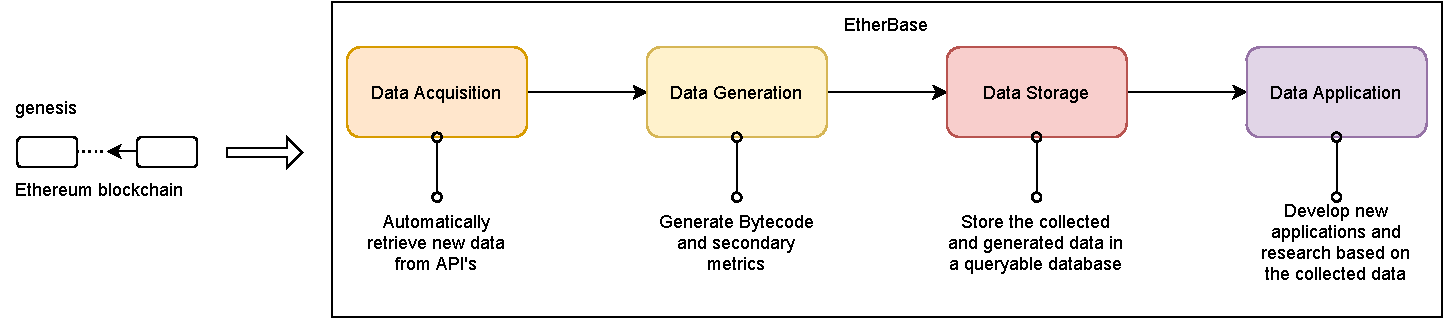
\includegraphics[width=1\textwidth]{figures/Untitled Diagram.pdf}
		\caption{EtherBase Worflow}
		\label{fig:my_label}
	\end{figure}
	
	We specifically designed \etherbase to not provide the end-users with a dump of contracts and their corresponding features in a vague file hierarchy.
	We have a service offering the ability to filter and analyze smart contracts and a dataset of smart contracts with interesting features to conduct empirical research on, according to metrics like Pragma version, ETH value, etc.
	To fulfill its purpose, \etherbase is designed to perform four primary automatic operations on the data:
	\begin{enumerate}
		\item \textbf{Data Acquisiton}: Automatic retrieval of off-chain and on-chain data
		\item \textbf{Data Generation}: Generation of bytecode and other metrics
		\item \textbf{Data Storage}: Storage of the collected data in a public and accessible way
		\item \textbf{Data Application}: Development of new applications and research based on the available database
	\end{enumerate}

	The next sections walk through the above-mentioned steps of the workflow one-by one.

	\subsection{Data Acquisition}
		The current dataset is collected from Etherscan, which is the largest decentralized platform for Ethereum smart contracts.
		Every contract stored on Etherscan's database is indexed by its own corresponding addresses,
		In order to collect these smart contracts, We first retrieve the addresses for every contract which has more than one transaction through Google BigQuery.
		Using Google BigQuery query request service, we obtain 1,712,347 distinct contract addresses that have more than one transactions associated with them.

	\subsection{Data Generation}
		Instead of writing scripts to obtain the bytecode and/or source code thrpugh Etherscan's API, we leverage a tool designed and maintained by Trail of Bits, namely Cyitic-compile.
		All the previous works of research, work on providing either source code or bytecode of smart contracts to the researchers, but that will not be enough for the users who want to compile the smart contracts or build tools upon such data.
		Compiling smart contracts is also a tricky busines, due to the rapid pace of changing versions of the dominant programming language, Solidity, used to write and develop smart contracts.
		We developed crytic-compile, a library to help the compilation of smart contracts, to help with this problem.
		It helps the user to be needless of maintaining an interface with solc and it automatically finds and uses the right version of solc or a better compatiable version of solc to compile the input smart contracts.
		They way this works under the hood is that crytic-compile compiles an input smart contract and outputs a compilation untit in the standard solc output format, written in a json file, alongside the source code and other metadata.
		Unlike the other proposed datasets and tools discussed in Section~\ref{sec:relwork}, EtherBase targets the core problem of the lack of reproducibility in the research literature.
		Discussions surrounding what types of secondary metrics to retrieve from the Ethereum blockchain or third-party services will be explored further.
		
		For the rest of the analysis of the collected contracts, we only get to work on contracts with available source-code.
		We adopt the method used in the work of ~\cite{deduplicate} to remove the duplicates smart contracts,
		that is checking the MD5 checksums of each of the two source files in the collected dataset to see if they are the same and after removing the whitespace among the lines of code.
		After the process of deduplication is done, we get down to 48,622 smart contracts contracts.
		For this paper and as of now, we have released 5,000 smart contracts for the tool comparison purposes.
		There exist many metrics that we have access to, can calculate, and add to \etherbase, but not a lot of research has been conducted on the applicability
		of these many different types of metrics to empirical research on the Ethereum blockchain or how much it appeals to the researchers active in this field.
		In the following, we describe the initial set of the metrics we selected to include in EtherBase in the form of a table, to be followed by more,
		after more discussion and research on their applicability to research on smart contracts.

		The built-in metrics relating to smart contracts are those features which depend on the internal properties of a smart contract, e.g. SLOC (Source Lines of Code), Pragma version, number of modifiers, payable, etc. Hence the title \emph{primary metrics}.

		For this table, we decided to include the core metrics of a smart contract, which would help a researcher collect a large set of smart contracts rapidly, and conduct further analysis on them, comprising of:

		\begin{table}[H]
			\caption{Primary Metrics on Smart Contracts}
			\label{tab:intrinsic-cues}
			\centering
			\begin{adjustbox}{width=1\textwidth}
			\def\arraystretch{1.3}
			\begin{tabular}{l|p{105mm}}
				\textbf{Name} & \textbf{Description} \\
				\hline
				\verb|Pragma| & The \verb|pragma| keyword is used to enable certain compiler features or checks.\\
				\verb|Contract Address| & Unique 20-byte address, used as the main index to distinguish smart contracts from each other. \\
				\verb|Creator Address| & Indicates the address of the deeployer of the smart contract. \\
				\verb|Source Code| & Source code of the smart contract, specific to the programming language Solidity. \\
				\verb|Bytecode (bin)| & . \\
				\verb|Bytcode (bin-runtime)| & . \\
				\verb|ABI| & The content of the application binary interface for each contract. \\
				\verb|Block Number| & The length of the blockchain in blocks. \\
				\verb|ETH Value| & The value of each smart contract in therms f=of the ETH thay hold. \\
				\verb|Transaction Count| & Number of internal transactions from eacch smart contract. \\
				%\verb|Deployer Status| & Indicates whether the deployer of a contract is a contract or not. \\
			\end{tabular}
			\end{adjustbox}
	\end{table}

	As for the primary metrics, here are our justifications for the above selection:

	\begin{itemize}

		\item{\verb|Pragma|: Source files can (and should) be annotated with a version pragma to reject compilation with future compiler versions that might introduce incompatible changes. Filtering through contracts via Pragma helps the researcher to collect a homogenuous set of contracts with a consistent synatx.}\\

		\item{\verb|Contract Address|: In Ethereum, the state is made up of objects called "accounts", with each account having a 20-byte address. Contract address is the main key in EtherBase for distinguishing contracts from each other.}\\

		\item{\verb|Creator Address|: The contract address is usually given when a contract is deployed to the Ethereum Blockchain. The address comes from the creator's address, where the contract has been initially deployed from, alongside the number of transactions sent from that address (the “nonce”). A creator's address can be helpful in analyzing the clone ratio and }\\

		\item{\verb|Source Code|: The source code of each Ethereum smart contract is written in Solidity and helps researchers do all sortds of analysis on the smart contracts.}\\

		\item{\verb|Bytecode (bin)|: The regular \verb|bin| output is the code placed on the blockchain plus the code needed to get this code placed on the blockchain, the code of the constructor.}\\

		\item{\verb|Bytecode (bin-runtime)|: \verb|bin-runtime| is the code that is actually placed on the blockchain.}\\

		\item{\verb|ABI|: \verb|ABI| stands for application binary interface. It's basically how you can encode Solidity contract calls for the EVM and, backwards, how to read the data out of transactions.}\\

		\item{\verb|Block Number|: \verb|Block Number|is the length of the blockchain in blocks, more specifically the block on which the smartt contract exists.}\\
		\item \verb|ETH Value|: The ETH every smart contract hols is an excellent filter or bar to select "interesting" contracts through for further research on the contracts that are more \emph{active} on the blockchain.\\

		\item \verb|Transaction Count|: Like ETH Value, transaction count is an important metric for us to be able to exclude contracts that do not participate much on the chain and hence, work on the contracts thast have a higher probability of interaction with more contracts.\\
		\end{itemize}
	
		\subsection{Data Storage}
			In the data storage stage, all extracted data are stored in PostgreSQL-alongside a GitHub repository- for the ease of data management.
			Users can get access to the collected data in PostgreSQL.
			In the application stage, users can conduct various analyses on the collected data.

			Figure 2 shows the directory structure of the collected data. The first leaf in the directory \texttt{Contracts} corresponds to the \\


\definecolor{folderbg}{RGB}{124,166,198}
\definecolor{folderborder}{RGB}{110,144,169}

\def\Size{4pt}
\tikzset{
  folder/.pic={
    \filldraw[draw=folderborder,top color=folderbg!50,bottom color=folderbg]
      (-1.05*\Size,0.2\Size+5pt) rectangle ++(.75*\Size,-0.2\Size-5pt);  
    \filldraw[draw=folderborder,top color=folderbg!50,bottom color=folderbg]
      (-1.15*\Size,-\Size) rectangle (1.15*\Size,\Size);
  }
}
\resizebox{0.6\textwidth}{!}{%
\begin{forest}
  for tree={
    font=\ttfamily,
    grow'=0,
    child anchor=west,
    parent anchor=south,
    anchor=west,
    calign=first,
    inner xsep=7pt,
    edge path={
      \noexpand\path [draw, \forestoption{edge}]
      (!u.south west) +(7.5pt,0) |- (.child anchor) pic {folder} \forestoption{edge label};
    },
    before typesetting nodes={
      if n=1
        {insert before={[,phantom]}}
        {}
    },
    fit=band,
    before computing xy={l=15pt},
  }  
[contracts
  [0
  ]
  [1
    [0
      [0
        [0
          [0
            [5
              [0x100005bc082d49eefffdc720864984bd7f3f7e5e
                [0x100005bc082d49eefffdc720864984bd7f3f7e5e-SudEX.sol
                ]
                [artifact.zip
                ]
                [slither-findings.json
                ]
                [slither-findings.md
                ]
                [slither-findings.txt
                ]
              ]
            ]
          ]
          [...
          ]
          [f
          ]
        ]
        [...
        ]
        [f
        ]
      ]
      [...
      ]
      [f
      ]
    ]
    [...
    ]
    [f
    ]
  ]
  [...
  ]
  [f
  ]
]
\end{forest}
}%
\newline
The \texttt{artifact.zip} file contains

\resizebox{0.3\textwidth}{!}{%
\begin{forest}
  for tree={
    font=\ttfamily,
    grow'=0,
    child anchor=west,
    parent anchor=south,
    anchor=west,
    calign=first,
    edge path={
      \noexpand\path [draw, \forestoption{edge}]
      (!u.south west) +(7.5pt,0) |- node[fill,inner sep=1.25pt] {} (.child anchor)\forestoption{edge label};
    },
    before typesetting nodes={
      if n=1
        {insert before={[,phantom]}}
        {}
    },
    fit=band,
    before computing xy={l=15pt},
  }
[\texttt{objects}
  [\texttt{compilation\_units}
    [contract.sol
        [compiler]
        [asts]
        [contracts
            [contracts.sol
                [abi]
                [bin]
                [bin-runtime]
                [srcmap]
                [srcmap-runtime]
            ]
            [SafeMath]
            [...]
        ]
    ]
  ]
]
\end{forest}
}%

	In addition to making the datasets available on GitHub, \etherbase also enjoy a graphical user interface (GUI) in order to allow the less technical end users access
	and browse through the database.
	We integrated \etherbase with Apache Superset, a powerful business intelligence tool, which lets you creata charts and dashboards using the data from the database.

\subsection{Data Application}
	In order to showcase an application of the empirical usage of the data from \etherbase, 
	the 5,000 filtered smart contract data set is labelled using three of the most prominently used static analysis tools in Ethereum research that detect
	various vulnerabilities in smart contracts, using a majority voting mechanism, in order to see how they fare against each other based an automatically labelled dataset.
	The criteria we used for tool selection was pretty simple; we wanted tools that had a focus on assessing Solidity source code instead of bytecode,
	and that they are available as open-source software and can be evaluated based on their vulnreability detection mechanisms.
	Based on such criteria, we selected the following three tools for our Data Application phase experiment:
	\begin{itemize}
		\item \textbf{Slither:} Slither~\cite{slither} is a static analysis tool designed to analyze Ethereum smart contracts.
		It has four prominent use cases:
		automated detection of vulnerabilities, automated detection of code optimization opportunities, improvement of users' understanding of the contracts,
		and assistant with code review.
		\item \textbf{Mythril:} Mythril is a tool that does security analysis of Ethereum smart contracts. It detects various security issues~\cite{mythril}.
		\item \textbf{Smartcheck:} Smartcheck~\cite{smartcheck} is an extensible static analysis tool that detects vulnerabilities in smart contracts.
		It converts Solidity code into XML-based intermediate representation and checks it with XPATH patterns.
	\end{itemize}
	
	
	We select three of the highest ranked vulnerabilities according to the DASP 10 ranking by the NCC Group, to test the aforementioned tools based upon.
	The thre vulnerabilities, as explained in Chapter 2, are as follows:
	\begin{itemize}
		\item \textbf{Re-entrancy} also known as the recursive call vulnerability, with SWCRegistry ID SWC-107.
		\item \textbf{Arithemtic:} concerning the integer overflows and underflow vulnerabilities in smart contracts, with SWCRegistry ID SWC-101.
		\item \textbf{Unchecked Ether:} also known as or related to silent failing sends, which can lead to unexpected behavior if return values are not handled properly, with SWCRegistry ID SWC-104.
	\end{itemize} 
	
	\begin{table}[t]
		\caption{Supported Vulnerabilities}
		\label{tab:freq}
	   %\renewcommand{\arraystretch}{1.2}
		\begin{tabular}{cccc}
	  
	  \multirow{2}{*}{\textbf{Tool Name}} & \multicolumn{3}{c}{\textbf{Vulnerability Type}} \\
		 & ARTHM & RENT & UE \\ \midrule
		  Slither    & \crossmark  &  \checkmark  &  \checkmark  \\
		  Mythril    & \checkmark  &  \checkmark  &  \checkmark  \\
		  Smartcheck & \checkmark  &  \crossmark  &  \checkmark  \\
		  \bottomrule
	  \end{tabular}
	  \label{table:vuln_supported_per_tool}
	  \end{table}
	
	
	%Table \ref{table:vuln_supported_per_tool} shows these vulnerabilities supported by the selected tools.
	The \checkmark symbol shows that the tool can detect a particular vulnerability, whereas symbol \crossmark indicates that the tool can't detect the vulnerability.
	
	We use the methodology given in the paper by Ren et al.~\cite{Making-Smart-Contract-Development-More-Secure-and-Easier} to detect the selected vulnerabilities in smart contracts.
	
	Because of the presence of false positives in the reports generated by the static analysis tools, we cannot depend on just one of them.
	We use majority voting, that is, at least 50\% of the tools must report the same vulnerability at the same location.
	For example, assume that tools T1, T2, and T3 can detect the re-entrancy vulnerability.
	Suppose, at least two tools report that vulnerability is present in a smart contract in test.
	Then we say that the contract is vulnerable;
	Otherwise, we say that the contract is not vulnerable.
	
	The following steps explain the methodology given the majority voting mechanism explained above:
	
	\begin{enumerate}
	
	\item First, collect the output of the selected tools for the smart contract to be analyzed.
	
	\item Note the vulnerability name and line number for the vulnerability per tool. 
	
	\item For the same vulnerability, if different tools show different locations, consider them as different warnings.
		We consider two warnings as the same only if the vulnerability name and location match for different tools.
	
	\item The methodology says that the vulnerability exists at a location if more than 50\% of the tools (2 out of 3 in this experiment scenario) confirm the same vulnerability at the exact location.
		In that case, label the location with the vulnerability.
	
	\end{enumerate}
	
	\begin{figure}[t]
		\centering
		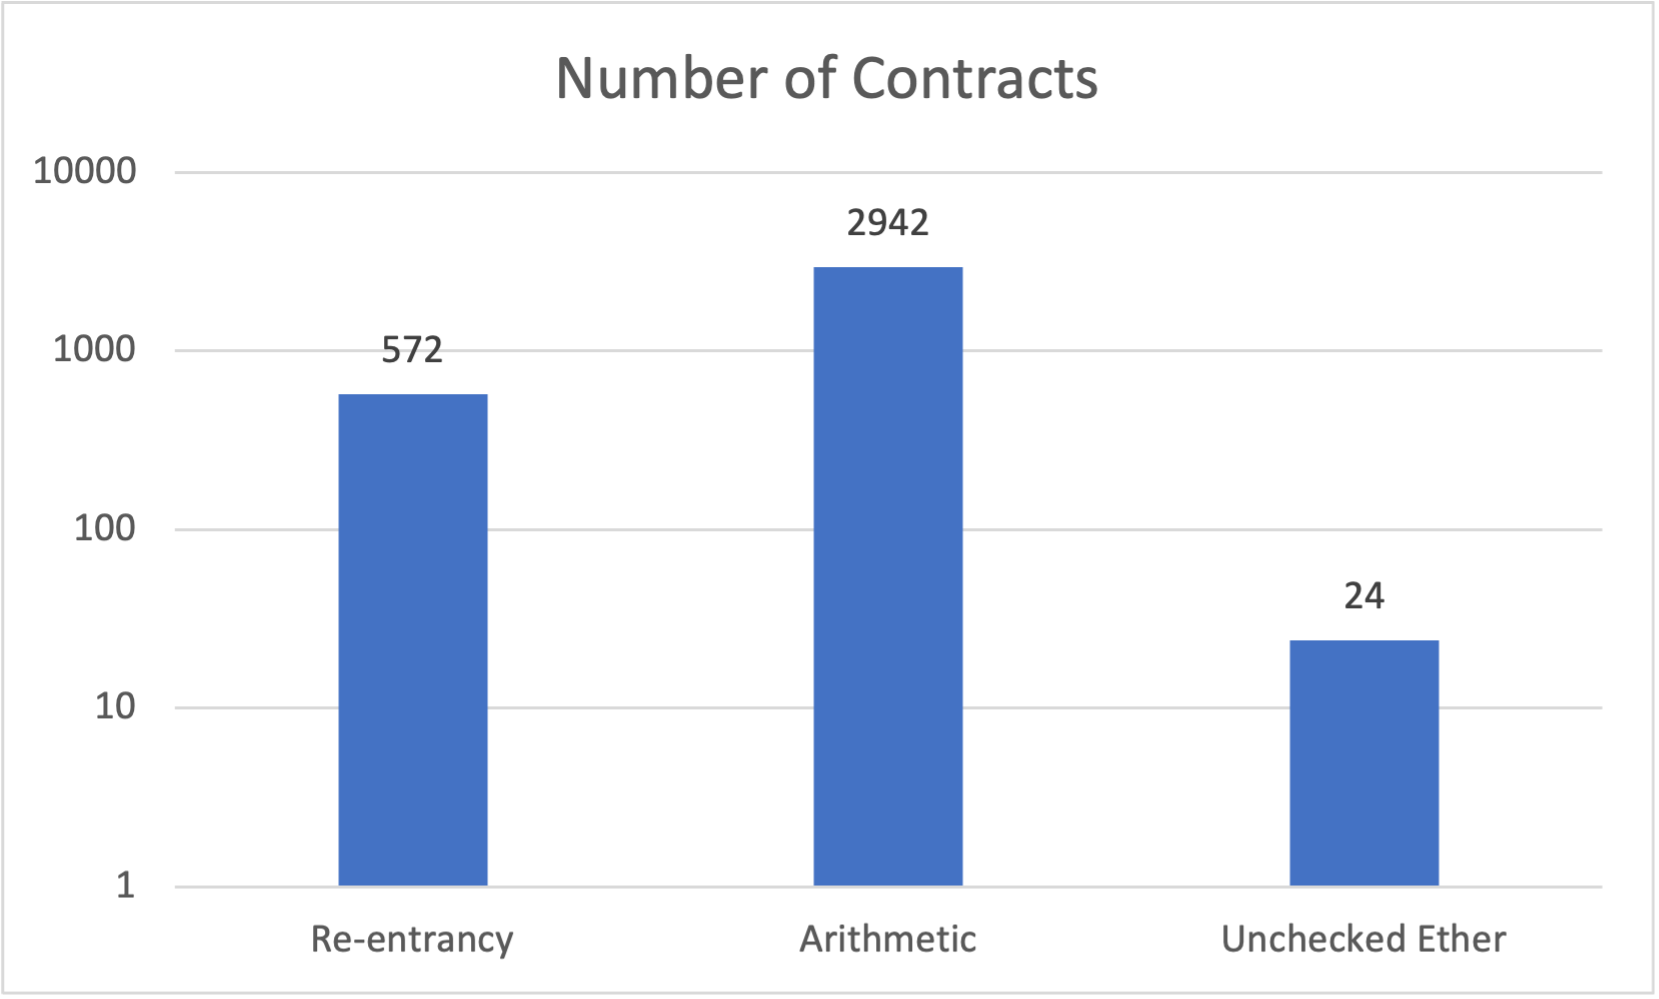
\includegraphics[width=1\textwidth]{figures/Picture1.png}
		\caption{No. of Contracts containing vulnerabilities (log-scale)}
		\label{fig:chart_vuln_count}
	\end{figure}
		
		Figure~\ref{fig:chart_vuln_count} shows the number of smart contracts that contain at least one vulnerability.
		For instance, consider the Re-entrancy vulnerability.
		The literature tells us that all fo the the three static analyzers in the benchmark support the detection of this vulnerability.
		We say that the contract contains reentrancy only if two of these three tools report that it is present at the same location.


\section{Concluding Remarks}
	This chapter introduces an up-to-date database, centred around Ethereum smart contracts, namely \etherbase, which includes data on the Ethereum blockchain (blocks),
	its smart contracts, and their metadata.
	Moreover, aggregate statistics and dataset exploration is presented.
	Furthermore, future research directions and opportunities are outlined:

	During the time we were building EtherBase, we utilized Web3 APIs without taking advantage of an Ethereum full / archive node.
	The next version of \etherbase we're already working on, will take full use of an Ethereum full node and instrment it in order to add a variety of more data to EtherBase.
	Collecting data via invoking Web3 API's is very much slower than instrumenting an Ethereum archive node.
	
	In addition, our current method is restricted by the rate limit imposed by the API's.
	For example, Etherescan restricts the frequency of invoking its API to 5 queries per second. We plan to solve this as well to speed the automated processes.

	We will also be labelling more smart contracts with more tools as we have more time and compute resources moving forward.

	The Ethereum security research community can use \etherbase for evaluating correctness and other parameters of their proposed or other toolsets,
	especially those based on machine learning techniques that need comprhensiver datasets for training, validation, and testing phases.
	\etherbase~comprises a diverse and comprehensive set of real-world heterogenuous annotated smart contracts.
	
	Every tool which was selected for this evaluation is not a complete one.
	There are always many false positive / negatives results generated by a static analyser.
	Nevertheless, we utilized the mechanism of majority voting to determine the presence or lacke of precense of a vulnerability in a smart contract.
	But, this approach may fail if majority of the tools generate false positives or false negatives.
	Such issues can be overcome by adding more tools to the benchamrk process or have some auditors manually review the discovered potential vulnerabilities..
	However, these approaches are time and resource-intensive, and we can plant to implement it incrementally.
%\include{chapters/chapter5/chapter5}


%%%%%%%%%%%%%%%%%%%%%%%%
\chapter{Conclusion and Future Work}
\label{chap:conclusion}

In this thesis, we presented \etherbase, an up-to-date database of Ethereum smart contracts to help researchers and developers use it as a testbed for evaluating and benchmarking various smart contracts security tools and frameworks.

Besides that, we provided an overview of the necessary background for someone with a background in electrical / computer engineering to realize the motivation behind providing such a dataset, with regards to the importance of the practice of mitigating vulnerabilities in smart contracts and the lackings in its ecosystem.

We went through the literature concerning the tools researchers have proposed to facilitate the discovery and mitigation of such vulnerabilities and explained how all of them lack the necessary benchmark and testing dataset for reproducibility for further research.

We proposed a version of \slithersimil~as the first machine-learning-based tool based on a static analysis tool and how it extended into developing \etherbase.

In the final chapter, we propose \etherbase: an up-to-date database of Ethereum smart contracts written in Solidity, to further facilitate further benchmarking and reproducibility in smart contract research.

%%%%%%%%%%%%%%%%%%%%%%%%%%%%%%%%%%%%%%%%%%%%%%%%
%% Bibliography
%%%%%%%%%%%%%%%%%%%%%%%%%%%%%%%%%%%%%%%%%%%%%%%%
\clearpage
\phantomsection
\addcontentsline{toc}{chapter}{Bibliography}  %  Add Bibliography to TOC
\singlespacing % save space in the bibliography
\bibliographystyle{abbrv}
\bibliography{references,bib/pulp.bib,bib/new.bib,bib/bib.bib}



%%%%%%%%%% Appendices %%%%%%%%%%%%%%%%
% ---- Appendix settings. Please Do NOT change them. -----
\appendix
\setcounter{table}{0}		% reset the table counter
\setcounter{figure}{0}		% reset the figure counter
\renewcommand{\thefigure}{\Alph{chapter}.\arabic{figure}} 	% numbering the a figure in Appendix as Figure A.2, Figure B.1, etc.
\renewcommand{\thetable}{\Alph{chapter}.\arabic{table}}		% numbering the a table in Appendix as Table A.2, Table B.1, etc.

%%%%%%%%%% Body of Appendix %%%%%%%%%%%%%%%%
%\begin{appendices}
%\doublespacing

%\chapter{First Appendix}
%\label{chap:apdx1}



%\chapter{Concordia Logos}
%\label{chap:logos}
%\begin{figure}[h!]
%	\centering
%	
\includegraphics{logos/Concordia_University_logo}
%	\caption{Concordia University}
%\end{figure}
%\vspace{2em}
%\begin{figure}[h!]
%	\centering
%	
\includegraphics{logos/Concordia_GinaCody_vertical}
%	\caption{Gina Cody School of Engineering and Computer Science (vertical)}
%\end{figure}
%\vspace{2em}
%\begin{figure}[h!]
%	\centering
%	
\includegraphics{logos/Concordia_GinaCody_horizontal}
%	\caption{Gina Cody School of Engineering and Computer Science (horizontal)}
%\end{figure}

%\end{appendices}

\end{document}